% arara: pdflatex: { shell: yes }
% arara: pythontex: {verbose: yes, rerun: modified }
% arara: pdflatex: { shell: yes }


\documentclass[study-guide-sol]{subfiles}
\externaldocument{study-guide}

\opt{solutionfiles,check}{
\Opensolutionfile{hint}
\Opensolutionfile{ans}
}

\begin{document}



\chapter{Chapter 7: Questions and remarks}
\label{cha:questions-chapter-7}


\section{Simple questions}

\subsection*{Section 7.1}


\begin{exercise}
In your own words, explain what is
\begin{enumerate}
\item a joint PMF, PDF, CDF;
\item a conditional PMF, PDF, CDF;
\item a marginal PMF, PDF, CDF.
\end{enumerate}
\begin{solution}
Check the definitions of the book.

Mistake: To say that $\P{X=x}$ is the PMF for a continuous random variable is wrong, because $\P{X=x}=0$ when $X$ is continuous.

Why is $\P{1 < x \leq 4}$ wrong notation?
hint: $X$ should be a capital.
What is the difference between $X$ and $x$?

\end{solution}
\end{exercise}

\begin{exercise}
Suppose  a head twice out of two coin flips is $\P{X_1=H, X_2=H}$.
hWat has this to do with joint PMFs? Can you generalize this idea to other examples?
\begin{solution}
This example shows why joint distributions are important!
Any experiment that involves a sequence of measurements, such as multiple throws of a coin, or the weighing of a bunch of chimpanzees, we have to deal with joint CDFs and PMFs.
\end{solution}
\end{exercise}


\begin{exercise}
In the previous exercise, suppose the outcome of the second throw is always equal to that of the first. Specify the joint PMF.
\begin{solution}
Here, we deal with two rvs, and we have to specify how they depend. In the present case $\P{X_1= H, X_2=H} = \P{X_1=H}$ and $\P{X_1= T, X_2=T} = \P{X_1=T}$, $\P{X_1= H, X_2=T} = \P{X_1= T, X_2=H} = 0$. Note that with this, we specified the joint PMF on all possible outcomes.
\end{solution}
\end{exercise}


\begin{exercise}
We have two rvs $X, Y \in [0,1]^{2}$ (here $[0,1]^{2} = [0,1]\times [0,1]$) with the joint PDF $f_{X,Y}(x,y) = 2 \1{x\leq y}$.
\begin{enumerate}
\item Are $X$ and $Y$ independent?
\item Compute $F_{X,Y}(x,y)$.
\end{enumerate}
\begin{solution}
\begin{align}
f_{X}(x) &= \int_{0}^{1} f_{X,Y}(x,y) \d y = 2\int_{0}^{1} \1{x\leq y} \d y = 2\int_{x}^{1} \d y = 2(1-x) \\
f_{Y}(y) &= \int_{0}^{1} f_{X,Y}(x,y) \d x = 2\int_{0}^{1} \1{x\leq y} \d x = 2\int_{0}^{y} \d y = 2 y.
\end{align}
But $f_{X,Y}(x,y) \neq f_{X}(x)f_{Y}(y)$, hence $X,Y$ are dependent.

\begin{align}
F_{X,Y}(x,y)
&= \int_{0}^{x}\int_{0}^{y} f_{X,Y}(u,v) \d v \d u \\
&= 2\int_{0}^{x}\int_{0}^{y} \1{u\leq v} \d v \d u \\
&= 2\int_{0}^{x}\int \1{u\leq v} \1{0\leq v \leq y}\d v \d u \\
&= 2\int_{0}^{x}\int  \1{u\leq v \leq y}\d v \d u \\
&= 2\int_{0}^{x} [y-u]^{+} \d u,
\end{align}
because $u\geq y \implies \1{u\leq v \leq y} = 0$. Now, if $y>x$,
\begin{align}
  2\int_{0}^{x} [y-u]^{+} \d u &=
  2\int_{0}^{x} (y-u) \d u = 2 y x - x^{2},
\end{align}
while if $y\leq x$,
\begin{align}
  2\int_{0}^{x} [y-u]^{+} \d u &=
  2\int_{0}^{y} (y-u) \d u = 2 y^{2} - y^{2} = y^{2}
\end{align}

Make a drawing of the support of $f_{X,Y}$ to help to understand this better.

\end{solution}
\end{exercise}

\begin{exercise}
We have two continuous rvs $X, Y$.
Suppose the joint CDF factors into the product of the marginals, i.e., $F_{X,Y}(x,y) = F_X(x)F_Y(y)$. Can it still be possible in general that the joint PDF does not factor into a product of marginals PDFs of $X$ and $Y$, i.e., $f_{X,Y}(x,y) \neq f_X(x) f_Y(y)$?
\begin{solution}
\begin{align*}
\partial_{x}\partial_{y}F_{X,Y}(x,y)
=\partial_{x}\partial_{y}F_{X}(x) F_{Y}(y)
=\partial_{x}F_{X}(x) \partial_{y} F_{Y}(y) = f_{X}(x) f_{Y}(y).
\end{align*}
\end{solution}
\end{exercise}

\begin{exercise}
BH define the conditional CDF given an event $A$ on page 416 as $F(y|A)$.
Use this definition to write $F_{X,Y}(x,y)/F_{X}(x)$ as a conditional CDF.
Is this equal to the conditional CDF of $X$ and $Y$?
\begin{solution}
\begin{align}
\frac{F_{X,Y}(x,y)}{F_{X}(x)} = \frac{\P{X\leq x, Y\leq y}}{\P{X\leq x}}
  = \P{Y\leq y, X\leq x|X\leq x} = \P{Y\leq y|X\leq x}.
\end{align}
It is a big mistake to write $F_{X,Y}(x,y) = \P{X=x, Y=y}$. If you wrote this, recheck the definitions of BH.
\end{solution}
\end{exercise}

\begin{exercise}
Let $X$ be uniformly distributed on the set $\{0,1,2\}$ and let $Y \sim \Bern{1/4}$; $X$ and $Y$ are independent.
\begin{enumerate}
\item Present a contingency table for $X$ and $Y$.
\item What is the interpretation of the column sums of the table?
\item What is the interpretation of the row sums of the table?
\item Suppose you would change some of the entries in the table. Are $X$ and $Y$ still independent?
\end{enumerate}
\begin{solution}
$\P{X=0, Y=0} = 1/3 \cdot 3/4$,
$\P{X=0, Y=1} = 1/3 \cdot 1/4$, and so on.

If we have one column with $Y=0$ and the other with $Y=1$, then the sum over the columns are $\P{Y=0}$ and $\P{Y=1}$. The row sum for row $i$ are  $\P{X=i}$.

Changing the values will (most of the time) make $X$ and $Y$ dependent. But, what if we changes the values such that  $\P{X=0, Y=0} =1$? Are $X$ and $Y$ then again independent? Check the conditions again.
\end{solution}
\end{exercise}

\begin{exercise}
A machine makes items on a day.
Some items, independent of the other items, are failed (i.e., do not meet the quality requirements).
What are $N$ and  $p$ in the context of the chicken-egg story of BH? What are the `eggs' in this context, and what is the meaning of `hatching'?
What type of `hatching' do we have here?
\begin{solution}
  The number of produced items (laid eggs) is $N$. The probability of hatching is $p$, that is, an item is ok. The hatched eggs are the good items.
\end{solution}
\end{exercise}

% \begin{exercise}
% Apply the chicken-egg story. Families enter a zoo in a given hour. Some families have one child, other two, and so on.
% What are the `eggs' in this context, and what is the meaning of `hatching'?
% \end{exercise}


\begin{exercise}
We have two rvs $X$ and $Y$ on $\R^{+}$. It is given that $F_{X,Y}(x,y) = F_X(x)F_Y(y)$ for $x,y \leq 1/3$. It is true that then  $X$ and $Y$ are necessarily independent.
\begin{solution}
For $X, Y$ to be independent, it is necessary that  $F_{X,Y}(x,y) = F_X(x)F_Y(y)$ for all $x,y$, not just one particular choice. (This is an example that satisfying a necessary condition is not necessarily sufficient.)
\end{solution}
\end{exercise}

\begin{exercise}
I select a random guy from the street, his height $X\sim\Norm{1.8, 0.1}$, and I select a random woman from the street, her height is $Y\sim\Norm{1.7, 0.08}$.
I claim that since I selected the man and the woman independently, their heights are independent.
Briefly comment on this claim.


\begin{solution}
  Many answers are possible here, depending on extra assumptions you make.
  Here is one.
  Suppose, just by change, the fraction of taller guys in the street is a bit higher than the population fraction.
  Assuming that taller (shorter) people prefer taller (shorter) spouses, there must be a dependence between the height of the men and the woman. This is because when selecting a man, I can also select his wife.

From this exercise you should memorize that \emph{independence is a property of the joint CDF, not of the rvs}.

Mistake:   $\P{Y}$ is wrong notation wrong because we can only compute the probability of an event, such as $\{Y\leq y\}$. But $Y$ itself is not an event. \end{solution}
\end{exercise}


\begin{exercise}
For any two rvs $X$ and $Y$ on $\R^{+}$ with marginals $F_{X}$ and $F_{Y}$, can  it hold that $\P{X\leq x, Y\leq y} = F_{X}(x) F_{Y}(y)$?
\begin{solution}
Only when $X, Y$ are independent.

Mistake:  independence of $X$ and $Y$ is not the same as the linear independence. Don't confuse these two types of dependene.
\end{solution}

\end{exercise}

\begin{exercise}
Theorem 7.1.11. What is the meaning of the notation $X|N=n$?
\begin{solution}
  Given $N=n$, the random variable $X$ has a certain distribution, here binomial.
\end{solution}
\end{exercise}

\begin{exercise}
Let $X, Y$ be two discrete rvs with CDF $F_{X,Y}$.  Can we compute the PDF as $\partial_{x}\partial_{y} F_{X,Y}(x,y)$?
\begin{solution}
This claim is incorrect, because $X, Y$ are discrete, hence they have a PMF, not a PDF.

Mistake: Someone said that $\partial_{x}\partial_{y}$ is not correct notation; however, it is correct! It's a (much used) abbreviation of the much heaver $\partial^{2}/\partial x \partial y$. Next, the derivative of the PMF is not well-defined (at least, not within this course. If you object, ok, but then show that you passed a decent course on measure theory.)
\end{solution}
\end{exercise}

\begin{exercise} Redo BH.7.1.24 with indicator functions and the  fundamental bridge (recall, $\P{A} = \E{\1{A}}$ for an event $A$).
(Indicators are often  easy to use, and prevent many mistakes, as is demonstrated with this example.)
\begin{solution}
\begin{align*}
\P{T_1 < T_2 } = \E{\1{T_1<T_2}} =
&= \int_0^\infty \int_0^\infty \1{t_1<t_2} f_{T_1, T_2}(t_1, t_2)\d t_{1} \d{t_2} \\
&= \int_0^\infty \int_{t_1}^{\infty}  \lambda_1 e^{-\lambda_1 t_1} \lambda_2 e^{-\lambda_2 t_2}  \d{t_2} \d{t_1}\\
&= \int_0^\infty   \lambda_1 e^{-\lambda_1 t_1} \lambda_2 \int_{t_1}^{\infty} e^{-\lambda_2 t_2}  \d{t_2} \d{t_1}\\
&= \int_0^\infty   \lambda_1 e^{-\lambda_1 t_1} e^{-\lambda_2 t_1}  \d{t_1}\\
&= \int_0^\infty   \lambda_1 e^{-\lambda_1 t_1 - \lambda_2t_{1}} \d{t_1}\\
&= \frac{\lambda_{1}}{\lambda_{1}+\lambda_2}.
\end{align*}
\end{solution}
\end{exercise}



\subsection*{Section 7.2}
\label{sec:section-7.2}


\begin{exercise}
BH.7.2.2. Write down the integral to compute $\E{(X-Y)^{2}}$, and solve it.
\begin{solution}
We have
\begin{align}
    \E{(X-Y)^2} &= \int_{-\infty}^\infty \int_{-\infty}^\infty (x - y)^2 f_{X,Y}(x,y) \d x \d y \\
    &=\int_0^1 \int_0^1 (x - y)^2 \d x \d y \\
    &=\int_0^1 \int_0^1 (x^{2} - 2 x y +  y^2) \d x \d y \\
    &=\int_0^1 \int_0^1 x^{2} \d x \d y
    -2\int_0^1 \int_0^1  x y  \d x \d y
    +\int_0^1 \int_0^1  y^2 \d x \d y  \\
    &=\int_0^1 x^{2} \d x
    -2\int_0^1 \int_0^1 x y  \d x \d y
    + \int_0^1  y^2  \d y \\
    &=1/3  -2 \cdot 1/ 2 \cdot 1/ 2 + 1/3.
\end{align}
\end{solution}
\end{exercise}


\begin{exercise}
Explain that for a continuous r.v. $X$ with CDF $F$ and $a$ and $b$ (so it might be that $a>b$),
\begin{equation}
  \label{eq:87}
\P{a< X < b} = [F(b) - F(a)]^{+}.
\end{equation}
\begin{hint}
  Recall that $F\in [0, 1]$.
\end{hint}
\begin{solution}
\begin{align}
a<b & \implies \P{a< X < b} = F(b) - F(a) = [F(b) - F(a)]^{+} \\
a\geq b & \implies \P{a< X < b} =  0 = [F(b) - F(a)]^{+},
\end{align}
where the last equality follows from the fact that $F$ is increasing.
\end{solution}
\end{exercise}

\begin{remark}
If you are like me, you underestimate at first the importance of using indicator functions. In fact, they are extremely useful for several reasons.
\begin{enumerate}
\item  They help to keep your formulas clean.
\item You can use them in computer code as logical conditions, or to help counting relevant events, something you need when numerically estimating multi-D integrals,  for machine learning for instance.
\item  Even though figures give geometrical insight into how to integrate over an 2D area, when it comes to reversing the sequence of integration, indicators are often easier to use.
\item In fact, \emph{expectation is the fundamental concept in probability theory}, and the \emph{probability of an event is defined} as
\begin{equation}
  \label{eq:84}
  \P{A} := \E{\1{A}}.
\end{equation}
Thus, the fundamental bridge is actually an application of LOTUS to indicator functions. Hence, reread BH.4.4!
\end{enumerate}
\end{remark}

\begin{exercise}
What is $\int_{-\infty}^{\infty} \1{0\leq x \leq 3} \d x$?
\begin{solution}
\begin{align*}
\int_{-\infty}^{\infty} \1{0\leq x \leq 3} \d x =\int_{0}^{3}  \d x  = 3.
\end{align*}
\end{solution}
\end{exercise}

\begin{exercise}
What is
\begin{equation}
\label{eq:85}
\int x \1{0\leq x \leq 4} \d x?
\end{equation}
\begin{solution}
\begin{align*}
\int x \1{0\leq x \leq 4} \d x  = \int_{0}^{4} x \d x = 16/2 = 8.
\end{align*}
\end{solution}
\end{exercise}

When we do an integral over a 2D surface we can first integrate over the $x$ and then over the $y$, or the other way around, whatever is the most convenient.
(There are conditions about how to handle multi-D integral, but for this course these are irrelevant.)

\begin{exercise}
What is
\begin{equation}
\label{eq:185}
\iint x y \1{0\leq x \leq 3}\1{0\leq y \leq 4} \d x \d y?
\end{equation}
\begin{solution}
\begin{align*}
\iint xy \1{0\leq x \leq 3}\1{0\leq y \leq 4} \d x \d y
&=\int_{0}^{3} x \int_{0}^{4} y \d y \d x\\
&=\int_{0}^{3} x \frac{y^{2}} 2 \biggr|_{0}^{4} \d x\\
&= \int_{0}^{3} x\cdot 8 \d x = 8\cdot 9/2 = 4\cdot 9.
\end{align*}
\end{solution}
\end{exercise}

\begin{exercise}
What is
\begin{align}
\label{eq:285}
\iint \1{0\leq x \leq 3} \1{0\leq y \leq 4}\1{x\leq y}\d x \d y?
\end{align}
\begin{solution}
Two solutions. First we integrate over $y$.
\begin{align}
\label{eq:385}
\iint \1{0\leq x \leq 3} \1{0\leq y \leq 4}\1{x\leq y}\d x \d y
&=\int \1{0\leq x \leq 3} \int \1{0\leq y \leq 4}\1{x\leq y}\d y \d x\\
&=\int \1{0\leq x \leq 3} \int \1{\max\{x, 0\} \leq y \leq 4}\d y \d x\\
&=\int_{0}^{3} \int_{\max\{x, 0\}}^{4}\d y \d x\\
&=\int_{0}^{3} y\biggr|_{\max\{x, 0\}}^{4} \d x\\
&=\int_{0}^{3}  (4-\max\{x, 0\}) \d x\\
&=12 - \int_{0}^{3} \max\{x, 0\} \d x\\
&=12 - \int_{0}^{3} x  \d x\\
&=12 - 9/2.
\end{align}

Let's now instead first integrate over $x$.
\begin{align}
\label{eq:485}
\iint \1{0\leq x \leq 3} \1{0\leq y \leq 4}\1{x\leq y}\d x \d y
&= \int \1{0\leq y \leq 4} \int \1{0\leq x \leq 3} \1{x\leq y}\d x \d y\\
&= \int_{0}^{4} \int \1{0\leq x \leq \min\{3, y\}}\d x \d y\\
&= \int_{0}^{4} \int_{0}^{\min\{3, y\}} \d x \d y\\
&= \int_{0}^{4} \min\{3, y\}\d y\\
&= \int_{0}^{3} \min\{3, y\}\d y + \int_{3}^{4} \min\{3, y\}\d y\\
&= \int_{0}^{3} y \d y + \int_{3}^{4}  3\d y\\
&= 9/2 + 3.
\end{align}
\end{solution}
\end{exercise}


\begin{exercise}\label{ex:2a}
Take $X\sim\Unif{[1,3]}, Y\sim\Unif{[2,4]}$ and independent. Compute
\begin{equation}
  \label{eq:824}
\P{Y\leq 2X}.
\end{equation}
\begin{solution}
Take $c$ the normalization constant (why is $c=1/4$), then using the previous exercise
\begin{align}
\P{Y\leq 2X}
&=\E{\1{Y\leq 2X}} \\
&=c \int_{1}^{3}\int_{2}^{4} \1{y\leq 2x} \d y \d x \\
&=c \int_{1}^{3}\int \1{2\leq y\leq \min\{4,2x\}}  \d y \d x \\
&=c \int_{1}^{3} [\min\{4, 2x\} -2]^{+} \d x
\end{align}
Now make a drawing of the function $[\min\{4, 2x\} - 2]^{+}$ on the interval $[1,3]$ to see that
\begin{equation}
\int_{1}^{3} [\min\{4, 2x\} -2]^{+} \d x = \int_{1}^{2} (2x -2) \d x + \int_{2}^{3} (4 -2) \d x.
\end{equation}
I leave the rest of the computation to you.
\end{solution}
\end{exercise}


\subsection*{Section 7.3}
\label{sec:section-7.3}



\begin{exercise}
Give a brief example of a situation where it might be more convenient to employ the correlation than the covariance.  Explain why.
\begin{solution}
The covariance might be a large number, which may  suggest that the rvs $X$ and $Y$ are `very' dependent. However, when $\V X$ and $\V Y$ are also large, the correlation can be small. Thus, correlation is a scaled type of covariance.
\end{solution}
\end{exercise}

\begin{exercise}
In queueing theory  the concept of squared coefficient of variance $SCV$ of a rv $X$ is very important. It is defined as $C = \V{X}/(\E X)^{2}$. Is the SCV of $X$ equal to $\text{Corr}(X,X)$? Can it happen that $C>1$?
\begin{solution}
Answers: no and yes.

We have
\begin{align}
    C = \frac{\V{X}}{(\E{X})^2},
\end{align}
which does not equal
\begin{align}
    \text{Corr}(X,X) = \frac{\cov{X,X}}{\sqrt{\V{X}\V{X}}} = 1
\end{align}
in general (for instance, consider a degenerate random variable $X \equiv 1$). Next, consider a $N(1,100)$ random variable. Then,
\begin{align}
    C = 100/(1^2) = 100 > 1.
\end{align}
\end{solution}
\end{exercise}


\begin{exercise}
Prove the key properties 1--5 of the covariance below BH.7.3.2.
\begin{solution}
\begin{enumerate}
    \item We have
    \begin{align}
        \cov{X,X} = \E{XX} - \E{X}\E{X} = \E{X^2} - \E{X}^2 = \V{X}.
    \end{align}
    \item We have
    \begin{align}
        \cov{X,Y} = \E{XY} - \E{X}\E{Y} = \E{YX} - \E{Y} \E{X} = \cov{Y, X}.
    \end{align}
    \item We have
    \begin{align}
        \cov{X,c} = \E{Xc} - \E{X}\E{c} = c\E{X} - c\E{X} = 0.
    \end{align}
    \item We have
    \begin{align}
        \cov{aX,Y} = \E{aXY} - \E{aX}\E{Y} = a\big(\E{XY} - \E{X}\E{Y}\big) = a\cov{X,Y}.
    \end{align}
    \item We have
    \begin{align}
        \cov{X+Y, Z} &= \E{(X + Y)Z} - \E{X+Y}\E{Z} \\
        &= \E{XZ + YZ} - \big(\E{X} + \E{Y}\big) \E{Z}\\
        &= \E{XZ} - \E{X}\E{Z} + \E{YZ} - \E{Y}\E{Z} \\
        &= \cov{X,Z} + \cov{Y,Z}.
    \end{align}
\end{enumerate}
\end{solution}
\end{exercise}

\begin{exercise}
Using the definition of Covariance (BH.7.3.1) derive the expression $\cov{X,Y}=\E{XY}-\E{X}\E{Y}$. Use this to show why independence of X and Y implies their uncorrelatedness (Note that the converse does not hold).
\begin{solution}
We have
\begin{align}
    \cov{X,Y} &= \E{(X - \E{X})(Y - \E{Y})} \\
    &= \E{XY - X\E{Y} - Y\E{X} + \E{X}\E{Y}} \\
    &= \E{XY} - \E{X}\E{Y} - \E{Y} \E{X} + \E{X}\E{Y}\\
    &= \E{XY}-\E{X}\E{Y}.
\end{align}
When $X$ and $Y$ are independent, then $\E{XY} = \E X \E Y$, and then $\cov{X,Y}=0$.
\end{solution}
\end{exercise}

\begin{exercise}
Let $U, V$ be two rvs and let $a,b\in \R$.
Using the previous question to express $\cov{a(U+V), b(U-V)}$ in terms of $\V{U}$, $\V{V}$ and $\cov{U,V}$.
\begin{solution}
By linearity of the covariance wea have
\begin{align}
    \cov{a(U+V), b(U-V)} &= a \Big( \cov{U, b(U-V)} + \cov{V, b(U-V)} \Big) \\
    &= a \Big( b\big( \cov{U, U} - \cov{U, V} \big)  + b\big( \cov{V, U} - \cov{V,V} \Big) \\
    &= a \Big( b\big( \cov{U, U} - \cov{U, V} \big)  + b\big( \cov{V, U} - \cov{V,V} \Big) \\
    &= a b \Big( \V{U} - \cov{U, V} + \cov{V, U} - \V{V} \Big) \\
    &= a b \Big( \V{U} - \V{V} \Big).
\end{align}
\end{solution}
\end{exercise}


\begin{exercise}\label{ex:3a}
The solution of BH.7.3.6 is a somewhat tricky; I would have not  found this trick myself. Here is an approach that is trick free.

Neglecting the event $\{X=Y\}$ as this has zero probability, we know that $M=X, L=Y$ or $M=Y, L=X$. Use this idea and the formula $\cov{M,L} = \E{ML} - \E M \E L$ to derive the result of this example.
\begin{hint}
Realize that $\E{ML} = \E{XY}$.
\end{hint}
\begin{solution}
With the hint: $\E{XY}=1/\lambda^{2}$, when $X, Y \sim\Exp{\lambda}$. Then, $L\sim \Exp{2\lambda}$, since $f_{L}(x) = 2 f_X(x) (1-F_Y(x)) = 2 \lambda e^{-2\lambda x}$. Therefore, $\E L = 1/2\lambda$. Also, by memoryless, $\E{M} = \E L + \E X = 3/2\lambda$. Hence, $\E{M}\E L = 3/4\lambda^{2}$. Hence, $\E{ML}- \E M \E L = 1/\lambda^{2-} 3/4\lambda^2 = 1/4\lambda^{2}$.
\end{solution}
\end{exercise}


\subsection*{Section 7.4}
\label{sec:section-7.4}

\begin{exercise}
Come up with a short illustrative example in which the random vector $\mathbf{X} = (X_1, \ldots, X_6)$ follows a Multinomial Distribution with parameters  $n=10$ and $\mathbf{p}=(\frac{1}{6}, ..., \frac{1}{6}) \in \R^{6}$.
\begin{solution}
We throw 10 fair dice. $X_i$ denotes the number of dice that show the number $i$, $i=1,\ldots,6$.
\end{solution}
\end{exercise}


\subsection*{Section 7.5}



\begin{exercise}
Is the following claim correct? If the rvs $X, Y$ are both normally distributed, then $(X, Y)$ follows a Bivariate Normal distribution.
\begin{solution}
No, this does not always hold, see BH.7.5.2. However, it does hold when $X$ and $Y$ are independent.
\end{solution}
\end{exercise}
\begin{exercise}
Let $X, Y, Z$ be iid $\mathcal{N}(0,1).$ Determine whether or not the random vector
\begin{align*}
    \mathbf{W} = (X+2Y, 3X+4Z, 5Y+6Z, 2X-4Y+Z, X-9Z, 12X+\sqrt{3}Y -\pi Z + 18)
\end{align*}
is Multivariate Normal. (Explain in words, don't do a lot of tedious math here!)
\begin{solution}
Since $X,Y,Z$ are independent normally distributed variables, $(X,Y,Z)$ is multivariate normally distributed. Hence, every linear combination of $X,Y,Z$ is normally distributed. Note that every linear combination of the elements of $W$ can be written as a linear combination of $X,Y,Z$. Hence, every linear combination of the elements of $W$ is normally distributed. Hence, $W$ is multivariate normally distributed.
\end{solution}
\end{exercise}


\subfile{memoryless_excursions.tex}


\section{Exercises on 2D integration}
\label{sec:exerc-2d-integr}

Here is some extra material for you practice on 2D integration, indicators and 2D LOTUS. These exercises are old exam questions, hence quite a bit harder than the above.  They form important training.

\begin{exercise}
Let $X$ and $Y$ be continuous random variables. Furthermore, $F(x,y)$ is the joint cumulative distribution function of $X$ and $Y$. This function has the following properties.
\begin{align*}\
    \begin{array}{lll}
        1. &F(x,y) = \dfrac{1}{8}(x-1)^2(y-2) & \text{for } 1< x<3 \text{ and  } 2< y< 4,\vspace{0.2cm}\\
        2. &\dfrac{\partial F(x,y)}{\partial x}=0& \text{for } x\notin (1,3),\vspace{0.2cm}\\
        3. &\dfrac{\partial F(x,y)}{\partial y}=0&\text{for } y\notin (2, 4).
    \end{array}
\end{align*}
Use these properties to answer the following questions.
\begin{enumerate}
\item  What is $F(2,5)$?
\item  Determine the joint probability density function of $X$ and $Y$.
\item  Determine $\text{P}(2<X<3,\, 2<Y<4)$.
\item  Determine the joint probability $\text{P}(Y<2X,\, 2X+Y>6)$. Clearly draw the area over which you integrate.
\end{enumerate}
\begin{solution}
a.  \begin{align*}
                F(2,5) = P(X\leq 2,Y\leq 5) = P(X\leq 2,Y\leq 4) = F(2,4) = \frac{1}{4}
    \end{align*}
    The second step is valid since the cumulative distribution function does not change by changing $y$ from 5 to 4 thanks to property 3.

b.             To obtain the joint pdf, use that $f_{X,Y}(x,y) = \dfrac{\partial^2}{\partial y\partial x}F(x,y) = \dfrac{\partial}{\partial y}\left(\dfrac{\partial}{\partial x} F(x,y)\right)$.\\
            Since
            $\dfrac{\partial}{\partial x} F(x,y) = \dfrac{1}{4}(x-1)(y-2)$ for $1< x < 3$, and $\dfrac{\partial}{\partial x} F(x,y) = 0$ for other values of $x$, we have that
            \begin{align*}
                f_{X,Y}(x,y) = \begin{cases}
                    \dfrac{1}{4}(x-1), & \mbox{for } 1<x<3 \mbox{ and } 2<y<4,\\
                    0, & \mbox{elsewhere}.
                \end{cases}
            \end{align*}

c.            The simplest way of solving this question is by writing
            \begin{align*}
                P(2<X<3,\, 2<Y<4) &= F(3,4) - F(2,4) - F(3,2) + F(2,2) \\
                &= 1 - \frac{1}{4} -0 + 0 = \frac{3}{4}.
            \end{align*}
            Alternatively, one can integrate over the pdf from (b) to obtain the same result:
            \begin{align*}
                P(2<X<3,\, 2<Y<4) &= \int_2^3\int_2^4f(x,y)\text{d}y\text{d}x\\
                &=\frac{1}{4}\int_2^3\left.(x-1)y\right|_{y=2}^{y=4}\text{d}x\\
                &=\frac{1}{4}\left(\left.x^2-2x\right|_2^3\right) = \frac{1}{4}\left(9-6-4+4\right) = \frac{3}{4}.
            \end{align*}


d.     First, draw the integration area:
            \begin{center}
                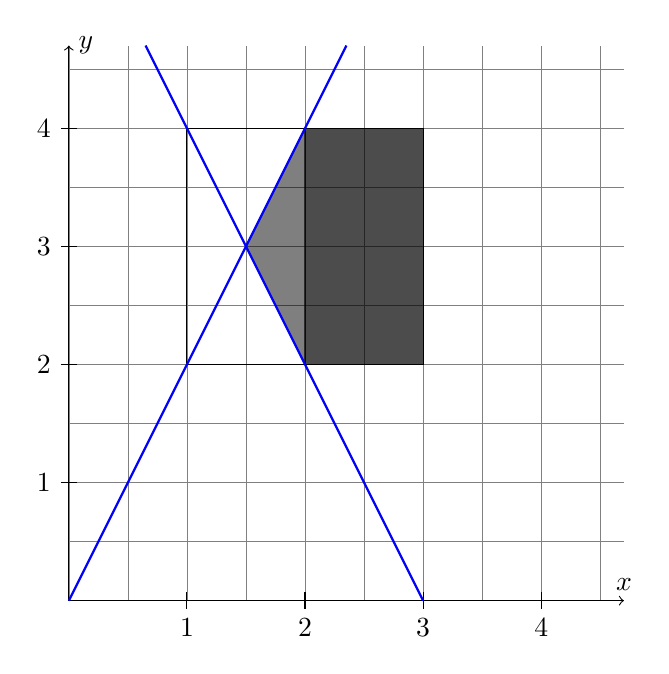
\begin{tikzpicture}[scale = 1.5]

                    \draw (1.05cm,2pt) node[above]{};
                    %  {$\displaystyle\int_0^{3/2} \!\!x^2\mathrm{d}x$};

                    \draw[style=help lines, step = 0.5] (0,0) grid (4.7,4.7);
                    % [step=0.25cm]      (1,2) grid +(1,1);

                    \draw[->] (0,0) -- (0,4.7) node[right] {$y$};
                    \draw[->] (0,0) -- (4.7,0) node[above] {$x$};
                    \foreach \x/\xtext in {1/1, 2/2, 3/3, 4/4}
                    \draw[shift={(\x,0)}] (0pt,2pt) -- (0pt,-2pt) node[below] {$\xtext$};

                    \foreach \y/\ytext in {1/1, 2/2, 3/3, 4/4}
                    \draw[shift={(0,\y)}] (2pt,0pt) -- (-2pt,0pt) node[left] {$\ytext$};

                    \draw[fill=black, fill opacity = 0]  (1,2) -- (1,4) -- (3,4) -- (3,2) -- cycle;
                    \draw[fill=black, fill opacity = 0.5]  (1.5,3) -- (2,4) -- (2,2);
                    \fill[black, fill opacity = 0.7] (2,4) -- (3,4) -- (3,2) -- (2,2);
                    \draw[domain=0.65:3,smooth,variable=\x,blue, thick] plot ({\x},{6-2*\x});
                    \draw[domain=0:2.35,smooth,variable=\x,blue, thick] plot ({\x},{2*\x});
                \end{tikzpicture}
            \end{center}
            The domain on which the density is non-zero, is the complete shaded area. The downward-sloping line represents $2x+y=6$ and the upward-sloping line is $y=2x$.

            We already know the integral over the dark shaded area from the previous subquestion. What remains is the lighter shaded triangular part on the left side.\\

                First, we need to calculate the intersection of the two curves, which can be found by solving $6-2x = 2x$, which gives $x= \frac{3}{2}$, and consequently $y = 3$.\\

            The integral of the triangular part of the dark shaded region is
            \begin{align*}
                \int_{3/2}^{2}\int_{6-2x}^{2x}\frac{1}{4}(x-1)dydx &= \int_{3/2}^{2}\left.\frac{1}{4}(x-1)y\right|_{6-2x}^{2x}dx\\
                &=\frac{1}{4}\int_{3/2}^{2}(x-1)2x-(x-1)(6-2x)dx\\
                &=\frac{1}{4}\int_{3/2}^{2}(x-1)(4x-6)dx\\
                &=\frac{1}{4}[\frac{4}{3}x^3-5x^2+6x]^{2}_{3/2}\\
                &=\dfrac{5}{48}\approx 0.1042\\
            \end{align*}
            Finally, the joint probability asked for in the question is given by
            $$P(Y<2X, 2X+Y>6) = \dfrac{5}{48}+\frac{3}{4} = \dfrac{41}{48}\approx 0.8542$$


\end{solution}
\end{exercise}

\begin{exercise}
 Suppose $X$ and $V$ are independent, $X\sim \text{Expo}(\lambda)$ and $V\sim \text{Expo}(\mu)$. Define the ratio $R=X/V$ and derive the cumulative distribution function (CDF) of $R$. Provide at least two checks on the CDF to make sure that your result is indeed a valid CDF.
    Note: There is no need to derive the probability density function (PDF) of $R$.
\begin{solution}
            For $r\geq 0$, we have
            \begin{align*}
                F_{R}(r)& = P(R\leq r) \\
                &= P(X\leq Vr)\\
                & = \int_{-\infty}^{\infty}\int_{-\infty}^{vr}f_{X,V}(x,v)dxdv\\
                & = \lambda\mu \int_{0}^{\infty}\int_{0}^{vr}e^{-\lambda x}e^{-\mu{v}}dxdv\\
                & = \lambda\mu\int_{0}^{\infty}e^{-\mu v}\left[-\frac{1}{\lambda}e^{-\lambda x}\right]_{0}^{vr}dv\\
                & = -\mu \int_{0}^{\infty}e^{-\mu v}(e^{-\lambda vr}-1)dv\\
                & = -\mu\left[-\frac{1}{\mu +\lambda r}e^{-(\mu+\lambda r)v}+\frac{1}{\mu}e^{-\mu v}\right]_{0}^{\infty}\\
                & = -\mu\left[\frac{1}{\mu+\lambda r}-\frac{1}{\mu}\right]\\
                & = \frac{\lambda r}{\mu+\lambda r},
            \end{align*}
            while $F_{R}(r)=0$ when $r<0$ since both $X$ and $V$ are nonnegative.

            We see that (1) $F_{R}(-\infty)=0$, (2) $F_{R}(\infty)=1$, and (3) $F_{R}(r)$ is monotonically increasing in $r$, so $F_{R}(r)$ satisfies the conditions for being a valid CDF.
\end{solution}
\end{exercise}


\begin{exercise}
 Consider the following joint density function
\begin{align*}
    f_{X,Y}(x,y) = \left\{\begin{array}{ll}
        cxy & \text{ for } 0\leq x<\frac{1}{2} \text{ and } 0\leq y\leq x,\\
        cxy & \text{ for } \frac{1}{2}\leq x\leq 1 \text{ and } 0\leq y\leq 1-x,\\
        0 & \text{otherwise.}
    \end{array}\right.
\end{align*}
\begin{enumerate}
\item  What is the correct value of the constant $c$?
\item Derive the conditional probability density function $f_{X|Y}(x|y)$. Verify that your result is indeed a valid density function.
\end{enumerate}

 \begin{solution}
a.         We integrate $f_{X,Y}(x,y)$ over its domain
        \begin{align*}
            &\int_{0}^{1/2}\int_{0}^{x}cxydydx + \int_{1/2}^{1}\int_{0}^{1-x}cxydydx\\
            = &c\left[\frac{1}{2}\int_{0}^{1/2}x^3dx + \frac{1}{2}\int_{1/2}^{1}x(1-x)^2dx\right]\\
            =&\frac{1}{2}c\left\{\left[\frac{1}{4}x^4\right]^{1/2}_{0} + \left[\frac{1}{2}x^2-\frac{2}{3}x^{3}+\frac{1}{4}x^{4}\right]^{1}_{1/2}\right\}\\
            & = \frac{1}{2}c\left\{\frac{1}{4}\frac{1}{16} + \frac{1}{2}-\frac{2}{3}+\frac{1}{4}-\frac{1}{2}\frac{1}{4} + \frac{2}{3}\frac{1}{8} - \frac{1}{4}\frac{1}{16}\right\}\\
            & = \frac{1}{2}c\frac{12-16+6-3+2}{24}\\
            & = \frac{c}{48}
        \end{align*}
        Since this integral should equal 1, $c = 48$. \newline\newline
        \textbf{Alternative} Rewrite the probability density function to
        \begin{align*}
            f_{X,Y}(x,y) = \left\{\begin{array}{ll}
                cxy & 0\leq y\leq \frac{1}{2},\quad y\leq x\leq 1-y\\
                0 & \text{otherwise}
            \end{array}\right.
        \end{align*}
        Then,
        \begin{align*}
            \int_{0}^{1/2}\int_{y}^{1-y}cxydxdy& = c\int_{0}^{1/2}y\frac{1}{2}\left((1-y)^2-y^2\right)\\
            & = \frac{1}{2}c\int_{0}^{1/2}\left( y-2y^2\right)dy\\
            &=\frac{1}{2}c\left[\frac{1}{2}y^2-\frac{2}{3}y^3\right]_{0}^{1/2}\\
            &=\frac{1}{2}c\left[ \frac{1}{8}-\frac{2}{3}\frac{1}{8}\right]
            =\frac{c}{48}
        \end{align*}
        Since this integral should equal 1, $c = 48$.


 b.
        The conditional density function is given by
        \begin{align*}
            f_{X|Y}(x|y) = \frac{f_{X,Y}(x,y)}{f_{Y}(y)}
        \end{align*}
        We first need the marginal density of $Y$.
        \begin{align*}
            f_{Y}(y)& = 48\int_{y}^{1-y}xydx\\
            & = 48y\left[\frac{1}{2}(1-y)^2-\frac{1}{2}y^2\right]\\
            &=24y\left[1-2y+y^2-y^2\right]\\
            &=24y(1-2y)\quad\text{for } 0\leq y\leq \frac{1}{2}
        \end{align*}
        and $f_{Y}(y)=0$ otherwise.
        \hrule\vspace{0.2cm}
        \textit{Not required}: We can check that this is a valid density function:
        \begin{align*}
            \int_{0}^{1/2}24y(1-2y)dy &= 24\left[\frac{1}{2}y^2-\frac{2}{3}y^3\right]^{1/2}_{0}\\
            & = 24\left[\frac{1}{2}\frac{1}{4}-\frac{2}{3}\frac{1}{8}\right]^{1/2}_{0}\\
            &=1
        \end{align*}
        \hrule\vspace{0.2cm}

b. Now we can obtain the conditional density function
        \begin{align*}
            f_{X|Y}(x|y) &=\frac{f_{X,Y}(x,y)}{f_{Y}(y)}\\
            &= \frac{48xy}{24y(1-2y)} = \frac{2x}{1-2y} \quad \text{for } y\leq x\leq 1-y, \text{ and } 0\leq y<\frac{1}{2}
        \end{align*}
        and $f_{X|Y}(x|y)=0$ otherwise. \newline\newline
        This is a valid density function since $f(X|Y)(x|y)\geq 0$, and
        \begin{align*}
            \int_{y}^{1-y}f_{X|Y}(x|y)dx & = \frac{2}{1-2y}\left[\frac{1}{2}x^2\right]^{1-y}_{y}\\
            &=1
        \end{align*}
\end{solution}
\end{exercise}

\begin{exercise}
 Suppose the random variables $X$ and $Y$ have the joint probability density function
\begin{align*}
    f_{X,Y}(x,y) = \left\{\begin{array}{cl}
        2 & \text{if } 0\leq x< 1,\quad  |y|<\frac{1}{2}(1-x),\\
        0 & \text{otherwise}
    \end{array}\right.
\end{align*}

\begin{enumerate}
\item Calculate the marginal probability density functions $f_{X}(x)$ and $f_{Y}(y)$ and show that these are valid probability density functions.
\item Find the conditional expectation $\text{E}[X|Y=y]$. Provide at least one `sanity check' that shows that your answer makes intuitive sense.
    If you did not find an answer to (a), you can use that
    \begin{align*}
        f_{Y}(y) = \left\{\begin{array}{ll}
            2(1-2|y|)&\text{ if } -\frac{1}{2}< y<\frac{1}{2},\\
            0 & \text{ otherwise}.
        \end{array}\right.
    \end{align*}
\item Calculate the joint cumulative distribution function $F_{X,Y}(x,y)$ for $x=\frac{1}{2}$ and $y=3$.
\end{enumerate}


\begin{solution}
a.             The joint PDF is nonzero above the red-shaded area in the following graph. (draw, draw, draw!)
            \begin{center}
                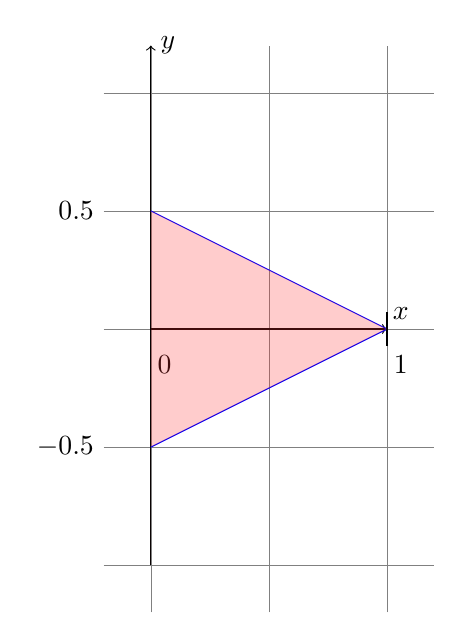
\begin{tikzpicture}[scale = 3]

                    \draw (1.05cm,2pt) node[above]{};
                    %  {$\displaystyle\int_0^{3/2} \!\!x^2\mathrm{d}x$};

                    \draw[style=help lines, step = 0.5] (-0.2,-1.2) grid (1.2,1.2);
                    % [step=0.25cm]      (1,2) grid +(1,1);

                    \draw[->] (0,-1) -- (0,1.2) node[right] {$y$};
                    \draw[->] (0,0) -- (1,0) node[above] {$\quad x$};
                    \draw[domain=(0):1,smooth,variable=\x,blue] plot ({\x},{0.5-0.5*\x});
                    \draw[domain=(0):1,smooth,variable=\x,blue] plot ({\x},{0.5*\x-0.5});
                    \foreach \x/\xtext in {0/0, 1/1}
                    \draw[shift={(\x,0)}] (0pt,2pt) -- (0pt,-2pt) node[below] {$\quad\xtext$};

                    \foreach \y/\ytext in {-0.5/-0.5,0.5/0.5}
                    \draw[shift={(-0.2,\y)}] node[left] {$\ytext$};

                    %		\draw[fill=red]  (0,11) -- (3,8) -- (3,4) -- (0,7) -- cycle;
                    %				\draw [dashed] (0,0.5) -- (0.75,0.5) node[right] {$\left(\frac{3}{4},\frac{1}{2}\right)$};
                    %				\draw [dashed] (0.75,0)-- (0.75,0.5);
                    %				\fill[red!20, nearly transparent]
                    %				[domain=0:0.5,smooth,variable=\x] (0,1) -- plot
                    %				({\x},{\x}) -- (1,1);
                    \fill[red!80, nearly transparent]
                    [domain=0:1,smooth,variable=\x] (0,-1) -- plot ({\x},{0.5*(\x-1)}) -- (0,0);
                    \fill[red!80, nearly transparent]
                    [domain=0:1,smooth,variable=\x] (0,1) -- plot ({\x},{0.5*(1-\x)}) -- (0,0);
                    % \fill[gray!20] (0,11) -- (0,12) -- (3,12) -- (3,8) -- cycle; %without transparency
                \end{tikzpicture}
            \end{center}

For the PDF  for $Y$,             using the graph above,
            \begin{align*}
                f_{Y}(y) &= \int_{-\infty}^{\infty}f_{X,Y}(x,y)dx\\
                & = \int_{0}^{1-2|y|}2dx\\
                & = 2(1-2|y|)\quad\text{for } -1/2< y< 1/2,
            \end{align*}
            and 0 otherwise.
            Since $-1/2< y< 1/2$, we have $f_{Y}(y)\geq 0$. Also,
            \begin{align*}
                \int_{-\infty}^{\infty}f_{Y}(y)dy &= \int_{-1/2}^{1/2}2(1-2|y|)dy\\
                &=2\int_{0}^{1/2}(1-2y)dy + 2\int_{-1/2}^{0}(1+2y)dy\\
                &=2\left(\frac{1}{2}-\frac{1}{4} +\frac{1}{2}-\frac{1}{4}\right) = 1.
            \end{align*}

Probability density function for $X$.
            \begin{align*}
                f_{X}(x) & = \int_{-\infty}^{\infty}f_{X,Y}dy\\
                & = \int_{-\frac{1}{2}(1-x)}^{\frac{1}{2}(1-x)}2dy\\
                & = 2(1-x)\quad\text{for } 0\leq x< 1,
            \end{align*}
            and 0 otherwise.
            We have $f_{X}(x)\geq 0$, and also
            \begin{align*}
                \int_{-\infty}^{\infty}f_{X}(x)dx &= \int_{0}^{1}2(1-x)dx\\
                &=2\left[x-\frac{1}{2}x^2\right]_{0}^{1}\\
                & = 2\left(1-\frac{1}{2}\right) = 1.
            \end{align*}
            Since $-1/2< y< 1/2$, we have $f_{Y}(y)\geq 0$. Also,
            \begin{align*}
                \int_{-\infty}^{\infty}f_{Y}(y)dy &= \int_{-1/2}^{1/2}2(1-2|y|)dy\\
                &=2\int_{0}^{1/2}(1-2y)dy + 2\int_{-1/2}^{0}(1+2y)dy\\
                &=2\left(\frac{1}{2}-\frac{1}{4} +\frac{1}{2}-\frac{1}{4}\right) = 1.
            \end{align*}

Probability density function for $X$.
            \begin{align*}
                f_{X}(x) & = \int_{-\infty}^{\infty}f_{X,Y}dy\\
                & = \int_{-\frac{1}{2}(1+x)}^{\frac{1}{2}(1+x)}2dy\\
                & = 2(1+x)\quad\text{for } -1< x\leq 0,
            \end{align*}
            and 0 otherwise.
            We have $f_{X}(x)\geq 0$, and also
            \begin{align*}
                \int_{-\infty}^{\infty}f_{X}(x)dx &= \int_{-1}^{0}2(1+x)dx\\
                &=2\left[x+\frac{1}{2}x^2\right]_{-1}^{0}\\
                & = 2\left(1-\frac{1}{2}\right) = 1.
            \end{align*}

b.
            Using the definition of a conditional probability density function, we have
            \begin{align*}
                f_{X|Y}(x|y) = \frac{f_{X,Y}(x,y)}{f_{Y}(y)}=\frac{1}{1-2|y|}\quad\text{for }-\frac{1}{2}<y<\frac{1}{2}, 0<x<1-2|y|
            \end{align*}
            and $0$ otherwise.


            The required expected value is (bounds are crucial!)
            \begin{align*}
                \text{E}[X|Y=y] = \int_{0}^{1-2|y|}\frac{x}{1-2|y|}dx = \frac{1}{2}(1-2|y|).
            \end{align*}
            If $y=-1/2$ or $y=1/2$, we find $\text{E}[X|Y=y]=0$, which makes sense based on the figure above. Similarly, if $y=0$, we find $\text{E}[X|Y=y] = 1/2$ since the density of $x$ is uniform over $[0,1]$.


            The point ($\frac{1}{2},3$) is located as in the picture below. We need to integrate $f_{X,Y}(x,y)$ over the entire area on the lower left side of this point. It is crucial to realize that the joint PDF is only nonzero in the red shaded area. Moreover, it's very helpful that the PDF has a constant value of 2 above this area.
            So we just need to calculate the the area of the red shape in the following graph and multiply this by 2.
            \begin{center}
                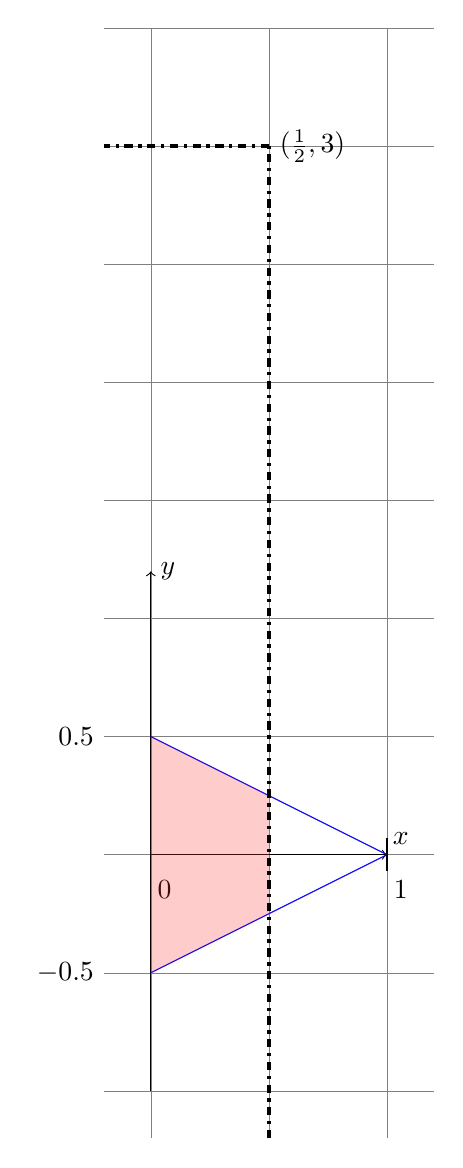
\begin{tikzpicture}[scale = 3]
                    \draw (1.05cm,2pt) node[above]{};
                    %  {$\displaystyle\int_0^{3/2} \!\!x^2\mathrm{d}x$};

                    \draw[style=help lines, step = 0.5] (-0.2,-1.2) grid (1.2,3.5);
                    % [step=0.25cm]      (1,2) grid +(1,1);

                    \draw[->] (0,-1) -- (0,1.2) node[right] {$y$};
                    \draw[->] (0,0) -- (1,0) node[above] {$\quad x$};
                    \draw[domain=(0):1,smooth,variable=\x,blue] plot ({\x},{0.5*(1-\x)});
                    \draw[domain=(0):1,smooth,variable=\x,blue] plot ({\x},{0.5*(\x-1)});
                    \foreach \x/\xtext in {0/0, 1/1}
                    \draw[shift={(\x,0)}] (0pt,2pt) -- (0pt,-2pt) node[below] {$\quad\xtext$};

                    \foreach \y/\ytext in {-0.5/-0.5, 0.5/0.5}
                    \draw[shift={(-0.2,\y)}] node[left] {$\ytext$};

                    \fill[red!80, nearly transparent]
                    [domain=0:1,smooth,variable=\x] (0.5,-0.25) -- (0.5,0.25) -- plot ({\x},{0.5*(1-\x)}) -- (0,0.5) -- (0,-0.5) -- plot ({\x},{0.5*(\x-1)});
                    \draw [very thick, dash dot] (0.5,-1.2) -- (0.5,3) node[right] {$(\frac{1}{2},3)$};
                    \draw [very thick, dash dot] (0.5,3) -- (-0.2,3);
                    % \fill[gray!20] (0,11) -- (0,12) -- (3,12) -- (3,8) -- cycle; %without transparency
                \end{tikzpicture}
            \end{center}
            The dash dotted line intersects the line $y = \frac{1}{2}(1-x)$ at $x=\frac{1}{2}$, so $y=\frac{1}{4}$. The line intersects $y=-\frac{1}{2}(1-x)$ at $x=\frac{1}{2}$, so $y=-\frac{1}{4}$.
            The whole area of the triangle is $\frac{1}{2}$. The area \textit{not} in red is $\frac{1}{2}\cdot(\frac{1}{4}-(-\frac{1}{4}))\cdot (1-\frac{1}{2}) = \frac{1}{8}$. So\
            \begin{equation*}
                F_{X,Y}\left(\frac{1}{2},3\right) =2\left(\frac{1}{2}-\frac{1}{8}\right)=\frac{3}{4}.
            \end{equation*}
\end{solution}
\end{exercise}


\begin{exercise}
Suppose the joint probability density function of $X$ and $Y$ is given by
\begin{equation*}
    f_{X,Y}(x,y) = \frac{c}{1-x}, \quad 0<x+y<1, \quad x>0, \quad y>0
\end{equation*}
and $f_{X,Y}(x,y)=0$ otherwise.
\begin{enumerate}
\item
For what value of the constant $c$ is $f_{X,Y}(x,y)$ a joint probability density function?
\item     What is the probability that $X+Y>\frac{1}{2}$?
\item     What is the probability that both $X$ and $Y$ are smaller than $\frac{1}{2}$ given that $X+Y>\frac{1}{2}$?
\end{enumerate}
\begin{solution}
a.        $f_{X,Y}(x,y)$ is a joint probability density function if
        \begin{enumerate}
            \item If $f_{X,Y}(x,y)$ satisfies
            \begin{align*}
                \int_{-\infty}^{\infty}\int_{-\infty}^{\infty}f_{X,Y}(x,y)dxdy = 1
            \end{align*}
            \item $f_{X,Y}(x,y)\geq 0$ for all $x$ and $y$.
        \end{enumerate}

        We have
        \begin{align*}
            \int_{-\infty}^{\infty}\int_{-\infty}^{\infty}f_{X,Y}(x,y)dydx& = \int_{0}^{1}\int_{0}^{1-x} \frac{c}{1-x}dydx \\
            &= c\int_{0}^{1}\frac{1-x}{1-x}dx = 1
        \end{align*}
        So to satisfy condition (1), we need to set $c=1$. \newline
        Check Condition (2): $f_{X,Y}(x,y)\geq 0$ for all $x,y$. \newline
        For $0<x<1$, $f_{X,Y}(x,y)> 0$. Outside of this interval $f_{X,Y}(x,y)=0$. So, we have that $f_{X,Y}(x,y)\geq 0$ for all $x,y$.\newline
        %	\textit{Correct integral limits, but calculation error leading to the wrong constant: -1 point.\newline
        %		 Forgetting to check whether $f_{X,Y}(x,y)\geq 0$, do not subtract points.}

b.         The following graph is used for questions $b$ and $c$.
        \begin{center}
            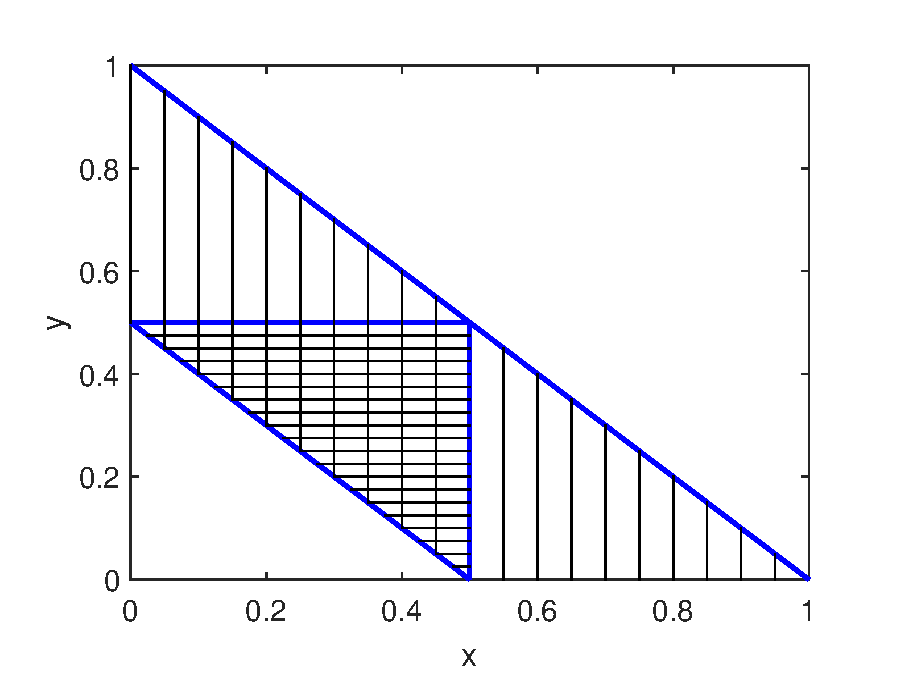
\includegraphics[width = 0.7\textwidth]{figures/pie.eps}
        \end{center}
        To obtain $P(X+Y>1/2)$, we need to integrate $f_{X,Y}$ over the vertically hatched area. We do this by integrating over the larger triangle defined by $x+y<1$, and then subtract the white triangle in the lower left corner defined by $x+y<\frac{1}{2}$.
        \begin{align*}
            P\left(X+Y>\frac{1}{2}\right) &= \int_{0}^{1}\int_{0}^{1-x}\frac{1}{1-x}dydx - \int_{0}^{1/2}\int_{0}^{1/2-x}\frac{1}{1-x}dydx\\
            & = 1-\int_{0}^{1/2}\frac{1/2-x}{1-x}dx\\
            & = 1-\int_{0}^{1/2}\left(1-\frac{1}{2}\frac{1}{1-x}\right)dx\\
            & = 1-\frac{1}{2} + \frac{1}{2}\int_{0}^{1/2}\frac{1}{1-x}dx\\
            & = \frac{1}{2}+\frac{1}{2}\left[-\ln(1-x)\right]^{1/2}_{0}\\
            & = \frac{1}{2}-\frac{1}{2}\ln\left(\frac{1}{2}\right)=0.8466
        \end{align*}
        %	\textit{Integrating over the wrong triangle: -2 points.\\
        %		Minor calculation errors: -1 point.\\
        %		Major calculation errors: -2 points.}


c.         Using the definition of conditional probability
        \begin{align*}
            P\left(X<\frac{1}{2},Y<\frac{1}{2}\left|X+Y>\frac{1}{2}\right.\right) = \frac{P\left(X<\frac{1}{2},Y<\frac{1}{2},X+Y>\frac{1}{2}\right)}{P\left(X+Y>\frac{1}{2}\right)}
        \end{align*}
        The integral in the numerator is the integral over the horizontally hatched triangle. Easiest is to first integrate over the square $[0,1/2]\times[0,1/2]$ and then subtract the lower white triangle, which we have already calculated in the previous question to be $\frac{1}{2}+\frac{1}{2}\ln\left(\frac{1}{2}\right)$.
        \begin{align*}
            \int_{0}^{1/2}\int_{0}^{1/2}\frac{1}{1-x}dydx & = \frac{1}{2}\int_{0}^{1/2}\frac{1}{1-x}dx\\
            & = \frac{1}{2}\left[-\ln(1-x)\right]^{1/2}_{0}\\
            & = -\frac{1}{2}\ln\left(\frac{1}{2}\right)
        \end{align*}
        Subtracting the lower triangle from the square, we see that the integral over the horizontally hatched triangle equals
        \begin{align*}
            -\frac{1}{2}\ln\left(\frac{1}{2}\right) - \frac{1}{2}-\frac{1}{2}\ln\left(\frac{1}{2}\right)=-\frac{1}{2}-\ln\left(\frac{1}{2}\right)
        \end{align*}
        We can then calculate
        \begin{align*}
            P\left(X<\frac{1}{2},Y<\frac{1}{2}|X+Y>\frac{1}{2}\right)=\frac{-\frac{1}{2}-\ln\left(\frac{1}{2}\right)}{\frac{1}{2}-\frac{1}{2}\ln\left(\frac{1}{2}\right)}\approx 0.23
        \end{align*}
        %	\textit{Integrating over the wrong triangle: -2 points.\\
        %		Minor calculation errors: -1 point.\\
        %		Major calculation errors: -2 points.}
\end{solution}
\end{exercise}


\begin{exercise}
 $X$ and $Y$ be random variables with joint probability density function
$$f_{X,Y}(x,y) = \begin{cases}
    \frac{3}{16}xy^2, & 0\le x\le c\mbox{ and } 0\le y\le c,\\
    0, & \mbox{elsewhere}
\end{cases}$$ where $c>0$ is a real number.
\begin{enumerate}
\item  Show that $c = 2$.
\item Show that $P(X+Y>2) = \frac{9}{10}$. Start by making a clear sketch of the area in the $(x,y)$-plane over which you take the required integral.
\item Calculate the conditional probability $P\left(\left.Y<X^2\right|X+Y<2\right)$.
\end{enumerate}
\begin{solution}
a.            Since $f_{XY}(x,y)$ is a joint probability density function, we should have\\
            1. $f_{X,Y}(x,y)\geq 0$. This is satisfied since $x,y\geq 0$. % \hfill \textbf{(1 point)}\\
            2.  $$\int_{-\infty}^{\infty}\int_{-\infty}^{\infty}f_{XY}(x,y)\text{d}x\text{d}y = 1,$$.
            We can calculate the integral as follows.
            \begin{alignat*}{3}
                \int_{-\infty}^{\infty}\int_{-\infty}^{\infty}f_{XY}(x,y)\text{d}x\text{d}y = 1\iff && \frac{3}{16}\int_{0}^{c}\int_{0}^{c}xy^2\text{d}x\text{d}y &= 1\\
                \iff && \frac{3}{32}\int_{0}^{c}\left(\left.x^2y^2\right|_0^c\right)\text{d}y &= 1\\
                \iff && \frac{3c^2}{32}\int_{0}^{c}y^2\text{d}y &= 1\\
                \iff && \left.\frac{3c^2}{96}y^3\right|_0^c &= 1\\
                \iff && 3c^5 &= 96
                \iff  c = 2 %\tag*{(\textbf{4 points})}
            \end{alignat*}

b. First, draw the area over which the integral is taken. %\hfill (\textbf{2 points})
            \begin{center}
                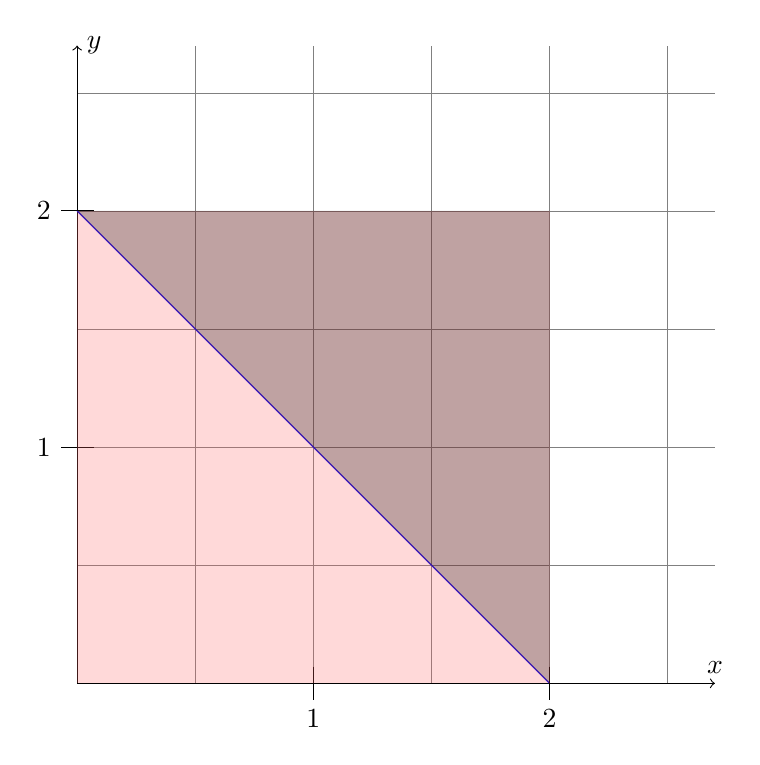
\begin{tikzpicture}[scale = 3]

                    \draw (1.05cm,2pt) node[above]{};
                    %  {$\displaystyle\int_0^{3/2} \!\!x^2\mathrm{d}x$};

                    \draw[style=help lines, step = 0.5] (0,0) grid (2.7,2.7);
                    % [step=0.25cm]      (1,2) grid +(1,1);

                    \draw[->] (0,0) -- (0,2.7) node[right] {$y$};
                    \draw[->] (0,0) -- (2.7,0) node[above] {$x$};
                    \draw[domain=(0):2,smooth,variable=\x,blue] plot ({\x},{2-\x});
                    \foreach \x/\xtext in {1/1, 2/2}
                    \draw[shift={(\x,0)}] (0pt,2pt) -- (0pt,-2pt) node[below] {$\xtext$};

                    \foreach \y/\ytext in {1/1, 2/2}
                    \draw[shift={(0,\y)}] (2pt,0pt) -- (-2pt,0pt) node[left] {$\ytext$};

                    %		\draw[fill=red]  (0,11) -- (3,8) -- (3,4) -- (0,7) -- cycle;
                    \fill[red!60, nearly transparent] (0,2) -- (2,2) -- (2,0) -- (0,0) -- cycle;
                    \fill[black, nearly transparent] [domain=0:2,smooth,variable=\x] plot ({\x},{2-\x}) -- (2,0) -- (2,2) -- (0,2);
                    % \fill[gray!20] (0,11) -- (0,12) -- (3,12) -- (3,8) -- cycle; %without transparency
                \end{tikzpicture}
            \end{center}

            We want to integrate over the darkest area. Hence, for every value of $y$, $x$ varies between $2-y$ and $2$. Hence, the required probability can be calculated as follows:\\
            \begin{minipage}[t]{0.45\textwidth}
                \textbf{Solution 1}
                \begin{align*}
                    &\quad P(X+Y>2)=\\
                    &= \int_{0}^{2}\int_{2-y}^{2}f_{X,Y}(x,y)\text{d}x\text{d}y\\
                    &= \frac{3}{16}\int_{0}^{2}\int_{2-y}^{2}xy^2\text{d}x\text{d}y\\
                    &= \frac{3}{32}\int_{0}^{2}\left(\left.x^2y^2\right|_{2-y}^2\right)\text{d}y\\
                    &= \frac{3}{32}\int_{0}^{2}(4y^2-(2-y)^2y^2)\text{d}y\\
                    &= \frac{3}{32}\int_{0}^{2}(4y^3-y^4)\text{d}y\\
                    &= \frac{3}{32}\left(\left.y^4-\frac{1}{5}y^5\right|_{0}^2\right)\\
                    &= \frac{3}{32}\left(16-\frac{32}{5}\right)\\
                    &= \frac{3}{2}-\frac{3}{5} = \frac{9}{10} %\tag*{(\textbf{3 points})}
                \end{align*}
            \end{minipage}
            \begin{minipage}[t]{0.45\textwidth}
                \textbf{Solution 2}
                \begin{align*}
                    &\quad P(X+Y>2)=\\
                    &= \int_{0}^{2}\int_{2-x}^{2}f_{X,Y}(x,y)\text{d}y\text{d}x\\
                    &= \frac{3}{16}\int_{0}^{2}\int_{2-x}^{2}xy^2\text{d}y\text{d}x\\
                    &= \frac{3}{16}\int_{0}^{2}\left(\left.\frac{1}{3}xy^3\right|_{2-x}^2\right)\text{d}x\\
                    &= \frac{1}{16}\int_{0}^{2}(8x-x(2-x)^3)\text{d}x\\
                    &= \frac{1}{16}\int_{0}^{2}(x^4+12x^2-6x^3)\text{d}x\\
                    &= \frac{1}{16}\left(\left.\frac{1}{5}x^5+4x^3-\frac{3}{2}x^4\right|_{0}^2\right)\\
                    &= \frac{1}{16}\left(\frac{32}{5}+32-24\right)\\
                    &= \frac{2}{5}+\frac{8}{16} = \frac{9}{10} %\tag*{(\textbf{3 points})}
                \end{align*}
            \end{minipage}
c. First, draw the area over which the integral is taken. % \hfill (\textbf{2 points})
            \begin{center}
                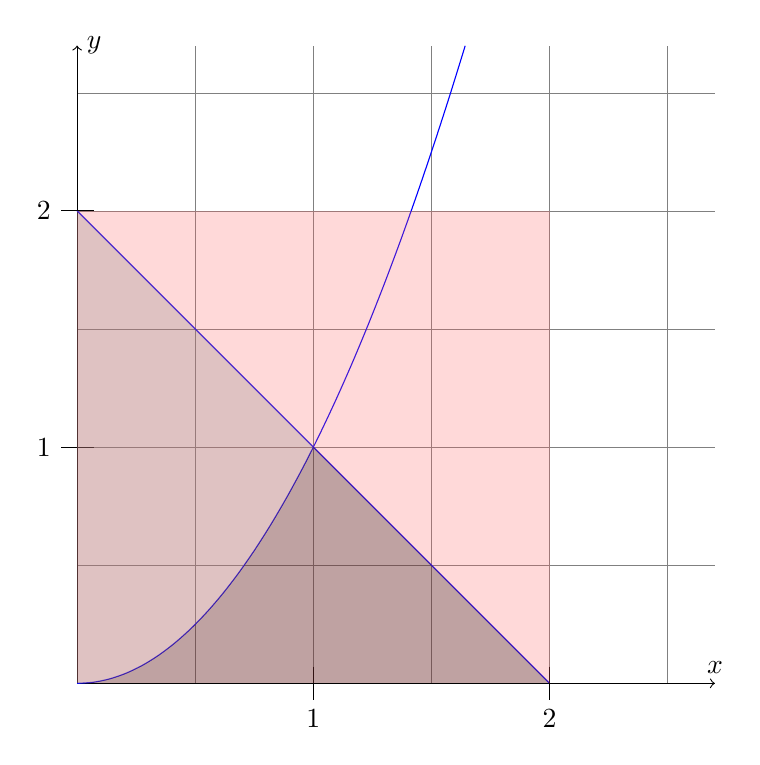
\begin{tikzpicture}[scale = 3]

                    \draw (1.05cm,2pt) node[above]{};
                    %  {$\displaystyle\int_0^{3/2} \!\!x^2\mathrm{d}x$};

                    \draw[style=help lines, step = 0.5] (0,0) grid (2.7,2.7);
                    % [step=0.25cm]      (1,2) grid +(1,1);

                    \draw[->] (0,0) -- (0,2.7) node[right] {$y$};
                    \draw[->] (0,0) -- (2.7,0) node[above] {$x$};
                    \draw[domain=0:2,smooth,variable=\x,blue] plot ({\x},{2-\x});
                    \draw[domain=0:sqrt(2.7),smooth,variable=\x,blue] plot ({\x},{\x*\x});
                    \foreach \x/\xtext in {1/1, 2/2}
                    \draw[shift={(\x,0)}] (0pt,2pt) -- (0pt,-2pt) node[below] {$\xtext$};

                    \foreach \y/\ytext in {1/1, 2/2}
                    \draw[shift={(0,\y)}] (2pt,0pt) -- (-2pt,0pt) node[left] {$\ytext$};

                    %		\draw[fill=red]  (0,11) -- (3,8) -- (3,4) -- (0,7) -- cycle;
                    \fill[red!60, nearly transparent] (0,2) -- (2,2) -- (2,0) -- (0,0) -- cycle;
                    \fill[black, nearly transparent] [domain=1:2,samples = 100,variable=\x] plot ({\x},{2-\x}) -- (2,0) -- (2,0) -- (1,0);
                    \fill[black, nearly transparent] [domain = 0:1, samples = 100, variable = \a] plot ({\a}, {\a * \a}) -- (1,1) -- (1,0) -- (0,0);
                    \fill[black!50, nearly transparent] [domain=0.5:1,samples = 100,variable=\x] plot ({\x},{2-\x}) -- (1,1) -- (0,1) -- (0,2) -- (0,2);
                    \fill[black!50, nearly transparent] [domain = 0:1, samples = 100, variable = \a] plot ({\a}, {\a * \a}) -- (0,1) -- (0,0);
                    % \fill[gray!20] (0,11) -- (0,12) -- (3,12) -- (3,8) -- cycle; %without transparency
                \end{tikzpicture}
            \end{center}

            The conditional probability is given by $$P(Y<X^2|X+Y<2) = \frac{P(X+Y<2\cap Y < X^2)}{P(X+Y<2)}.$$
            From part (b) we have $P(X+Y<2) = 1 - P(X+Y>2) = \frac{1}{10},$
            which means the probability of falling into one of the two darkest areas equals $\frac{1}{10}$. The probability $P(X+Y<2\cap Y < X^2)$ is given by the integral over the darkest area in the plot. \\
            \textbf{Solution 1}
            \begin{align*}
                P(X+Y<2\cap Y < X^2) &= \int_{0}^{1}\int_{0}^{x^2}f_{X,Y}(x,y)\text{d}y\text{d}x +\int_{1}^{2}\int_{0}^{2-x}f_{X,Y}(x,y)\text{d}y\text{d}x\\
                &= \frac{3}{16}\left[\int_{0}^{1}\int_{0}^{x^{2}}xy^2\text{d}y\text{d}x +\int_{1}^{2}\int_{0}^{2-x}xy^2\text{d}y\text{d}x\right]\\
                &= \frac{1}{16}\left[\int_{0}^{1}\left(\left.xy^3\right|_{0}^{x^{2}}\right)\text{d}x +\int_{1}^{2}\left(\left.xy^3\right|_{0}^{2-x}\right)\text{d}x\right]\\
                &= \frac{1}{16}\left[\int_{0}^{1}x^7\text{d}x +\int_{1}^{2}x(2-x)^3 \text{d}x\right]\\
                &= \frac{1}{16}\left[\int_{0}^{1}x^7\text{d}x +\int_{1}^{2}(-x^4+6x^3-12x^2+8x)\text{d}x\right]\\
                &= \frac{1}{128}\left[\left.x^8\right|_0^1\right] +\frac{1}{16}\left.\left(-\frac{1}{5}x^5+\frac{3}{2}x^4-4x^3+4x^2\right)\right|_{1}^{2}\\
                &= \frac{1}{128} + \frac{1}{16}\left(-\frac{32}{5}+24-32+16+\frac{1}{5}-\frac{3}{2}+4-4\right)= \frac{17}{640}
            \end{align*}
            \textbf{Solution 2 (easier)}
            \begin{align*}
                P(X+Y<2\cap Y < X^2) &= \int_{0}^{1}\int_{\sqrt{y}}^{2-y}f_{X,Y}(x,y)\text{d}x\text{d}y\\
                &= \frac{3}{16}\left[\int_{0}^{1}\int_{\sqrt{y}}^{2-y}xy^2\text{d}x\text{d}y\right]\\
                &= \frac{3}{32}\left[\int_{0}^{1}\left(\left.x^2y^2\right|_{\sqrt{y}}^{2-y}\right)\text{d}y\right]\\
                &= \frac{3}{32}\left[\int_{0}^{1}(2-y)^2 y^2 - y^3\text{d}y \right]\\
                &= \frac{3}{32}\left[\int_{0}^{1}4y^2-5y^3+y^4 \text{d}y\right]\\
                &= \frac{3}{32}\left[\left.\frac{4}{3}y^3-\frac{5}{4}y^4+\frac{1}{5}y^5\right|_0^1\right]\\
                &= \frac{3}{32}\left(\frac{4}{3}-\frac{5}{4}+\frac{1}{5}\right) = \frac{17}{640}
            \end{align*}

            Using either Solution 1 or Solution 2, we get the final answer:
            \begin{align*}
                P(Y<X^2|X+Y<2) = \frac{P(X+Y<2\cap Y < X^2)}{P(X+Y<2)} = \frac{\frac{17}{640}}{\frac{1}{10}} = \frac{17}{64}.
            \end{align*}
            %	\flushright{(\textbf{3 points})}
\end{solution}
\end{exercise}




\section{BH exercises: hints and solutions}
\label{sec:hints-solut-exerc}

% Exercises mentioned here are \emph{by default} obligatory to make.  Only if an exercise is marked as \emph{Optional}, it is optional.


\begin{exercise}
BH.7.1. We simulate this in one of the assignments.
\begin{hint}
Check BH 7.2.2. Bigger hint: Let $A$ the arrival time of Alice, and $B$ the time of Bob. Then we want to compute $\P{|A-B|\leq 1/4}$.  (15 minutes is 1/4 hour.)  Why is $f_{A,B}(a,b) = \1{a\in[0,1]}\1{b\in [0,1]}$? Now apply 2D-LOTUS to the function $g(a,b) = \1{|a-b|\leq 1/4}$.
\end{hint}
\begin{solution}
\end{solution}
\end{exercise}


\begin{exercise}
BH 7.9. We'll develop a simulation for this in the assignments.
\begin{hint}
a. $\P{X=i, Y=j, N=n} = \P{X=i, Y=j} \1{i+j=n}$.

c. $\P{X=i\given N=n} = 1/(n+1)$. Why is this uniform?
\end{hint}
\begin{solution}
Us the hint. For $k=0, 1, \ldots, n$,
\begin{equation*}
\P{X=k, N=n} = \P{X=k, Y=n-k} = pq^k p q^{n-k} = p^2 q^{n}.
\end{equation*}
(Have we used independence somewhere?)
Now observe that the right hand side does not depend on $k$. This implies that $\P{X=k|N=n}$  also does not depend on $k$. (Why?) But, since $\P{X=k|N=n}$ is a true PMF,  is must be that $\sum_{k=0}^{n}\P{X=k|N=n}$ adds up to $1$. These two ideas put together imply that $\P{X=k|N=n} = 1/(n+1)$.

With Bayes' expression
\begin{equation*}
\P{X=k|N=n} = \frac{\P{X=k, N=n}}{\P{N=n}},
\end{equation*}
it follows that
\begin{equation*}
\P{N=n} = \frac{\P{X=k, N=n}}{\P{X=k|N=n\P{N=n}}} = (n+1) p^2q^{n}.
\end{equation*}
\end{solution}
\end{exercise}

\begin{exercise} BH.7.10.

Recall that a conditional CDF given an event $A$ is defined as $F(y|A) = \P{Y\leq y|A}$. Likewise, let us write here $F_T(t|x) = \P{T\leq t|X=x}$.
Just use this in your derivation. However, there is one problem with the fact that the event $\{X=x\}$ has probablity zero. In the solution I'll discuss how to around this.

Don't forget to compare  this exercise to BH.7.9, which is the same but for discrete memoryless rvs.

\begin{solution}
Just reasoning as if there is no problem, i.e., applying Bayes' rule in a  naive way,
\begin{align*}
F_T(t|x) &= \P{T\leq t|X=x} = \P{X+Y\leq t|X=x} \\
  &=\P{Y\leq t-x, X=x}/\P{X=x} = \P{Y\leq t-x}\P{X=x}/\P{X=x}\\
  &=\P{Y\leq t-x}, 0\leq x \leq t.
\end{align*}
where I use that $Y$ and $X$ are independent to split the probability.

The problem with this derivation is that we multiply and divide by 0 ($=\P{X=x}$) just as if all is ok. But hopefully, you know that when we multiply and divide by zero, we can get any answer we like. A better way is as follows. Note beforehand that I do not expect that you could have  come up with such an answer, but you should definitely study it.


The first step is to realize that PDF $f_{T|X}(t|x)=f_{TX}(t,x)/f_X(x)$ \emph{is} well defined; we don't divide by zero because $f_{X}(x)>0$ on $x\geq 0$. By the proof of BH.8.2.1 we see that $f_{TX}(t,x) = f_X(x)f_Y(t-x) \1{0 \leq x \leq t}$, where I include the indicator to ensure that we don't run out of the support of $X$ and $T$. Thus,
\begin{align*}
  f_{T|X}(t|x) &= \frac{f_{TX}(t,x}{f_{X}(x)} = f_X(x)f_Y(t-x) \1{0 \leq x \leq t}/f_X(x) = f_Y(t-x)\1{0\leq x \leq t}.
\end{align*}
Now we know that a conditional PDF is a full-fledged PDF. So we can use idea that to \emph{define} the conditional CDF as follows:
\begin{align*}
F_{T|X}(t|x)
  := \int_0^t f_{T|X}(v|x)\1{0\leq x \leq v} \d v
    = \int_x^t \lambda e^{-\lambda(v-x)} \d v
    = \int_0^{t-x} \lambda e^{-\lambda v} \d v = 1- e^{-\lambda(t-x)}.
\end{align*}

Isn't it a bit strange that we get the same answer?
How to get out of this situation in a technically correct way is one of the hard parts of (mathematical) probability, and certainly not something we can deal with  in this course.
All books on elementary\footnote{When  in mathematics someething is elementary, it doesn't necessarily mean that that thing is simple. In fact, it can be very difficult.  Elementary means that we just dont use very advanced mathematical concepts.)} probability, and lecturers similarly, struggle with this problem; this course is not an exception, nor am I.

b.  See  part a.

c. By the above,
\begin{align*}
  f_{X|T}(x|t) &= f_{TX}(t,x)/f_T(t), \\
f_{TX}(t,x)  &=  f_X(x)f_Y(t-x) \1{0\leq x \leq t} \lambda^2 e^{-\lambda x} e^{-\lambda(t-x)} \1{0\leq x\leq t} = \lambda^2e^{-\lambda t} \1{0\leq x\leq t},\\
  &\implies  f_{X|T}(x|t) \propto \lambda^2e^{-\lambda t} \1{0\leq x\leq t} ,
\end{align*}
where the last follows because $f_T(t)$ is just a normalization constant.
Now we use some real nice, but subtle, reasoning to avoid computing $f_T$ by means of marginalizing out $x$ from $f_{T,X}(t, x)$.  Observe that $f_{TX}(t, x)$ is constant \emph{as a function of $x$} on $0\leq x \leq t$ (in other words, the RHS does not depend on $x$ on this interval). But $f_{X|T}(x|t)$  is also a real PDF. This implies  that the constant $f_T(t)$ (since it does not depend on $x$) must be  such that  $f_{X|T}(x|t)$ integrates to $1$ on $0\leq x \leq t$. The only possibility is that $f_{X|T}(x|t) = t^{-1}\1{0\leq x \leq t}$.

This reasoning gives some  offspin.  We can conclude that
\begin{align*}
  f_T(t) = f_{TX}(t, x)/f_{T|X}(t,x) = \lambda^2 t e^{-\lambda t}.
\end{align*}

This is more than a nice trick. Recall it, as it is not only used more often in the book, but also in more advanced courses on data science and machine learning.
\end{solution}
\end{exercise}


\begin{exercise}
BH.7.11
\begin{hint}
a.
First find $f_{Y|X}$ and $f{Z|X}$. Then, given $X$, $Z$ and $Y$ are iid. Hence $f_{X,Y,Z} = f_{Y, Z |X} f_{X}$. Use independence to split $f_{Y,Z|X}$ into a product.
b.
Suppose that $Y$ is really big. Since $Y$ is dependent on $X$, $X$ must be dependent on $Y$. But $Z$ is in turn dependent on $X$. What are the consequences?

\end{hint}
\begin{solution}
 c.
Here is the answer. The ideas are important, you'll need them during nearly any course in statistics, given the importance of the normal distribution.
\begin{align*}
f_{Y,Z}(y, z) = \int \frac 1 {2\pi} e^{-(y-x)^2/2} e^{-(z-x)^2/2} \frac 1 {\sqrt{2\pi}} e^{-x^2/2}\d x.
\end{align*}
It remains to simplify $(y-x)^2 + (z-x)^2 + x^2$. With a bit of work, it follows that this can be written as
\begin{align*}
3(x-(y+z)/3)^{2} - (y+z)^2/3+y^2+z^2.
\end{align*}
When plugging this in the integral, the last two terms appear in front of the integral. The term $(y+z)/2$ is just a shift, hence can be neglected in the integration over $x$. The $3$ has to be absorbed in the standard deviation $\sigma=1/\sqrt{3}$. And therefore,
\begin{align*}
f_{Y,Z}(y, z) = \frac 1 {2\pi} \frac 1 {\sqrt{3}} e^{-y^2/2 - z^2/2 + (y+z)^2/6}.
\end{align*}
\end{solution}
\end{exercise}

\begin{exercise}
BH.7.13
\begin{hint}
\cref{sec:memoryl-exerc-conf}
\end{hint}
\begin{solution}
\end{solution}
\end{exercise}

\begin{exercise}
BH7.15.
\begin{hint}
Make a drawing.
\end{hint}
\begin{solution}
Using the hint: $F(x,y)$ is the area of an (infinite) square lying  south west of the point $(x,y)$. Add and subtract such (infinite) squares until the square $[a_1,a_2] \times [b_{1},b_2]$ is covered exactly once. Realize that in the process, the square $(-\infty, a_1] \times (-\infty, b_1]$ is subtracted twice.
\end{solution}
\end{exercise}


\begin{exercise}
BH.7.24.
In the assignments we'll develop a simulator.

\begin{hint}
Check BH.7.1.24 and BH.7.1.25
First draw the area over which we have to integrate. Then use an indicator function over which to integrate. What is the joint PDF  $f_{Y_1, Y-2}$?
\end{hint}
\begin{solution}
From the hint,
\begin{align*}
\P{Y_1<c Y_2}
  &= \int \int \1{x<c y}\lambda_1 e^{-\lambda_1 x} \lambda_2e^{-\lambda_2 y}\d x \d y
  = \lambda_1\lambda_2\int_0^{\infty} e^{-\lambda_{1}x}\int_{x/c}^{\infty} e^{-\lambda_{2} y}\d y \d x\\
  & = \lambda_1\int_0^{\infty} e^{-\lambda_{1}x} e^{-\lambda_{2} x/c} \d x
  = \frac{\lambda_1}{\lambda_1+\lambda_2/c}.
\end{align*}
Check the result for $c=0$ and $c=\infty$.

I prefer to use conditioning, like this:
\begin{align*}
\P{Y_1<c Y_2}
  &= \int \P{Y_1<cY_2| Y_1=x}\lambda_1 e^{-\lambda_1 x} \d x
  = \int \P{Y_2>x/c| Y_1=x}\lambda_1 e^{-\lambda_1 x} \d x\\
&= \int e^{-\lambda x/c} \lambda_1 e^{-\lambda_1 x} \d x,
\end{align*}
and the rest goes as before. Actually, I tend to use conditioning as it helps to make the reasoning easier. In this case, suppose that I know that $Y_1=x$, what can I say about $\P{Y_2 > c x}$?

BTW, conditioning does not always make things simpler. When rvs are dependent, then you have to watch out.
\end{solution}
\end{exercise}


\begin{exercise}
BH.7.29
\begin{hint}
\cref{sec:memoryl-exerc-conf}
\end{hint}
\begin{solution}
\end{solution}
\end{exercise}


\begin{exercise}
BH. 7.38. Besides the solution of BH, read our solution.
\begin{solution}
First check~\cref{ex:3a}.

In general, I am always very careful with such `shortcuts' such as $\max\{X,Y\} + \min\{X, Y\} = X +Y$.  As a matter of fact, I try to avoid such arguments because it is easy to go wrong. Seemingly plausible arguments are often wrong due to overlooked dependency or non-linearity (effects of higher moments).

It is useful to write $\max\{x,y\} = x\1{x\geq y}+y\1{y>x}$, and something similar for the minimum. In the present case, $\cov{X,Y} = \E{X Y}-\E X \E Y$, and, similarly, $\cov{M,L} = \E{ML}- \E M \E L$, where $M$ is max, and $L$ is min. With the above indicators, it is simple to show that $\E{ML} = \E{X Y}$:
\begin{align*}
 ML
  &= (X\1{X\geq Y} + Y\1{Y\geq X})((X\1{X<Y} + Y\1{Y<X}) \\
  &= XY\1{X\geq Y} + XY\1{Y<X} = XY
\end{align*}
since $\1{X\geq Y}\1{X<Y} =0$.

However, take $X,Y\sim \Exp{\lambda}$. Then, $\E M = 3/(2\lambda)$ and $\E L= 1/(2\lambda)$, but $\E X = \E Y = 1/\lambda$.
\end{solution}
\end{exercise}

\begin{exercise}
BH.7.53. We simulate this in one of the assignments.
The ideas of this exercise find much use in finance, physics, and actuarial sciences.
In particular, the expected time it takes the drunken person---It's not only guys that sometimes consume too much alcohol---to hit some boundary is interesting. The notation of the book is a bit clumsy. Here is better notation.
Let $X_i$ be the movement along the \(x\)-axis at step $i$, and $Y_i$ along the $y$-axis.
Then $S_n=\sum_{i=1}^n X_i$ and $T_n=\sum_{j=1}^n Y_{j}$, and $R_n^2= S_n^2+T_n^2$.
\begin{hint}
Use the hint of the book and independence to see that $\E{S_{n}^2 T_n^2} = \E{S_n^{2}} \E{T_n^{2}}$.
Then try to simplify.

b. It is immediate that $\E{S_n} = 0$.
Hence, focus on $\E{S_n T_n}$. Expand  the sums of $\E{S_n T_n}$, and consider the individual terms $\E{X_i Y_j}$. When $i\neq j$, are $X_i$ and $Y_{j}$  independent? What if  $i=j$?

c. It is clear that $R_n^2=S_n^2+T_{n}^2$. Now use linearity to split $\E{R^2_n}$. Finally, realize that $\E{S_n}=0$, hence $\E{S_n^2} = \V{S_n}$. But then we can use the formula of the variance of a sum to split it up into a sum of variances plus covariances.
\end{hint}

\begin{solution}
a. In my notation, $X_i=0 \implies Y_i\neq 0$ and $X_i\neq 0 \implies Y_i=0$. The reason is that in step $i$, the drunkard makes a step left or right OR up or down. However, s/he cannot move to the right and up at the same time.

Here is an argument based on recursion. (By now I hope you see that I like this method in particular).
\begin{align*}
\E{R_n^2} = \E{(R_{n-1} + X_n + Y_n)^{2}},
\end{align*}
but $R_{n-1}$ and $X_n+Y_n$ are independent, and $\E{(X_n + Y_n)^2} = 1$. Using the recursion, $\E{R^2_n} = n$.
\end{solution}
\end{exercise}

\begin{exercise}
BH.7.58. This is a totally great exercise. First solve it yourself. In the solution, I'll explain why, in particular how to relate the concept of covariance to the determinant of a matrix.

\begin{hint}
a. Expand the brackets in the expression for the sample variance $r$ to see that
\begin{align*}
r = 1/n \sum_i x_i y_i - \bar x \bar y.
\end{align*}
Next, we choose with probability $1/n$ one the points $(x_i, y_{i})$.  Under this probability, $\E{X Y} = 1/n \sum_i x_i y_i$, $\E X = \bar x, \E Y = \bar y$. So, how do $\cov{X,Y}$ and $r$ relate?


b. Expand the brackets and use iid and linearity properties to show that the expected area spanned by two random points $(X,Y)$ and $(\tilde X, \tilde Y)$ satisfies
\begin{align*}
\E{(X-\tilde X)(Y-\tilde Y)} = 2\cov{X,Y}.
\end{align*}

\end{hint}
\begin{solution}

b. Use the hint. Then, if we choose two points at random from the sample, then $(x_i-x_j)(y_i-y_j)$ is the area spanned by these  two points.
More generally, I have $n$ choices for my first point, and also $n$ choices for the second point (if both points are the same, the area of the rectangle is 0, so we don't have to exclude such choices).
Hence, the expected area of the rectangle spanned by the two random points $(X,Y)$ and $(\tilde X, \tilde Y)$ is
\begin{align*}
\frac 1 {n^2} \sum_{i,j} (x_i-x_j)(y_i-y_j).
\end{align*}
Simplify this to show that
\begin{align*}
2 \frac 1 n \sum_i x_i y_i - 2 \bar x \bar y = 2 r
\end{align*}
Hence, by part a., the expected area is twice the covariance.

Why is $\cov{X,a}= 0$ for $a$ a constant? Because the `area' of rectangles, all with the same \(y\)-coordinate, is zero, i.e., they lie on a line.

c.  This is the part of the exercise that explains what the above is all about.
Since there is a direct relation between covariance and area, we can use geometric arguments to derive (and memorize!) all properties of covariance! Write property i. of covariance  as $\cov{X,Y} = \cov{Y,X}$. Suppose I flip the \(x\) and \(y\)-axis, does the area of a rectangle change?  For property ii., what happens to the area of rectangle if you stretch the sides? For property iii., realize that this is just a shift of a rectangle that leaves its area invariant. For property iv., what happens to the area if you put an extra rectangle on top or to the right?

BTW, property iii. follows directly from property iv. In iv., take $W_3$ equal to a constant $a_2$, in other words $\P{W_3=a_2}=1$. We know that $\cov{X, a} = 0$ for a constant $a$.

Here are  some final remarks.

Let's put all the above in a very general frame.  The covariance has a number of interesting properties:
\begin{enumerate}
\item  It is bilinear, that is, the covariance is linear in both arguments. The linearity in the first argument means that $\cov{X+Y, Z}=\cov{X,Z}+\cov{Y,Z}$ and $\cov{a X, Z}=a\cov{X,Z}$ for $a\in \R$. The linearity in the second argument means that $\cov{X, Y+Z}=\cov{X,Y}+\cov{X,Z}$ and $\cov{X, a Z}=a\cov{X,Z}$ for $a\in \R$.
\item It is symmetric: $\cov{X, Y}=\cov{Y,X}$, from which we define $\V X = \cov{X,X}$.
\item  $\cov{X,a} = 0$ for all $a\in R$.
\end{enumerate}
If you memorize the first two properties of covariance, all the rest follows.

Now we do some geometry. Take three vectors $x,y, z\in \R^2$ (it's easy to generalize to $\R^n)$. Then we know that the area $D(x,y)$ of the parallelogram spanned by vectors $x$ and $y$  satisfies the following properties.
\begin{enumerate}
\item  Area is bilinear. The linearity in the first argument means that $D(x+y, z) = D(x, z) + D(y, z)$ and $D(ax, z)=a D(x, z)$ for $a\in \R$. (Just make a drawing to convince you about this.) The linearity in the second argument means that  $D(x, y+z) = D(x, y) + D(x, z)$  and $D(x, a z)=a D(x, z)$ for $a\in \R$.
\item  $D(x,x)$ = 0; there is no area between $x$ and $x$.
\item $D( (1,0), (0,1)) = 1$; the area of the square with side 1 is 1.
\end{enumerate}
In fact, thex first property means that stretching vectors and stacking parallelograms result in stretching and adding areas.
The second says that the area of a parallelogram spanned by two parallel vectors is zero. The third specifies that the area of the unit square is 1.

Now it can be proven that there exists just one function $D$ that satisfies these properties. In fact, this is the determinant of the matrix with as columns the vectors that span the parallellogram. Moreover, it can be shown that the second property can be replaced by the skew-symmetric property: $D(x,y) = - D(x,y)$.
(Note that $D(x,x) = -D(x,x) \implies 2 D(x,x) = 0 \implies D(x,x) = 0$.)

Let us use the properties to compute the area of a parallelogram spanned by the vectors $x = (a,b)$ and $y =(c,d)$ in 2D. Then
\begin{align*}
D(x,y) &= D((a,b), (c,d)) =  D(a (1,0)) + b(0,1), c(1,0) + d(0,1)) \\
&= ad D((1,0), (0,1)) + b c D((0,1), (1,0)) = ad - b c,
\end{align*}
where we use bilinearity in the first step, and skew-symmetry in the second and third. And this is indeed the determinant of the matrix with $x$ and $y$ as columns.

So, all in all, this is what I remembered throughout the years: the covariance and the determinant are bi-linear forms, the first is symmetric, the second skew- (or anti-)symmetric.

Finally, I don't see why the areas of the rectangles have to have a sign in this problem. Interestingly, for the determinant, the areas of the parallelograms do have to have a sign to make the concept useful for physics.
\end{solution}
\end{exercise}

\begin{exercise}
BH.7.59.
Read this exercise, then read (and do) BH.5.53 for some further background.
You'll encounter these topics countless times in other courses!
The final answer is really nice and intuitive.

\begin{hint}
a. Use that expectation is linear.

b. Read the entire exercise in its entirety before trying to solve it. In this case trying to solve c.\/ seems simpler because of the extra iid assumption. You  might want to use this to formulate some simple guesses.

Thus first part c. It is given that the $X_i$ and $Y_j$ are iid. Then, if I could improve the estimator $\hat \theta$ by splitting the measurements into two sets $X_i$ and $Y_j$, then I would certainly do that.
And not only I would do that; anybody in his right mind would do that.
But, I never heard of this idea, and I am sure you have neither, so this must be impossible (because if it would, people would have been using this trick for ages.)
Hence, we can place this in the context of the maxim: `we cannot obtain information for free'.
For this case, this must imply that splitting iid measurements into smaller sets cannot help with improving the estimator. What does this idea imply for the weights?


Part b, continued. I always try to solve the problem myself without a hint. This lead to the following considerations, which gave me quite a bit of extra understanding beyond the problem itself.  As a next piece of advice, before doing hard work, I prefer to look at some corner cases to acquire some intuitive understanding. I also use the rvs of Part c.

Suppose  that $v_2:=\V{Y_j} = 0$, but $v_1 := \V{X_i} > 0$. (For instance, $Y_j$ is the $j$th measurement of a perfect machine and $X_j$ of an imperfect machine.)
Then we know that the set $\{Y_j\}$ forms a set of perfect measurements.
But then I am not interested in the $\{X_i\}$ measurements anymore; why should I as I have the perfect measurements $\{Y_j\}$ at my disposal.
So, then I put $w_1=0$, because I don't want the $\{X_i\}$ measurements to pollute my estimator.
In other words, the final result should be such that $v_2=0 \implies w_{1}=0$, and vice versa.


More generally, I learned from this  corner case that I want this for the final result:  when $v_2<v_{1} \implies w_1 < w_{2}$, and vice versa.

How would you choose the weights such that this requirement is satisfied, but also the condition imposed by Part c.?



\end{hint}


\begin{solution}
a. Follows directly from the hint.

Check the hint!

c.  If $X_i$ and $Y_j$ are iid, it must be that $w_{1} = n/(n+m)$.

b. Can we make some further progress, just by keeping a clear mind?
Well, in fact we can by using our insights of part c.
If we have $n+m$ iid measurements of which we call $n$ measurements of type $X_i$, and $m$ of type $Y_{j}$, then
\begin{align*}
\V{\hat \theta_{1}}  =  \E{\left(\frac{1}{n}\sum_{i}X_{i} - \theta\right)^2} = n^{-2}\E{\left(\sum_i (X_{i}-\theta)\right)^{2}} = n^{-2}\V{\sum_i X_i} = \V{X_1}/n = \sigma^{2}/n.
\end{align*}
So, $n=\sigma^{2}/\V{\hat \theta_1}$, and likewise $m=\sigma^{2}/\V{\hat \theta_2}$. Finally, plug this into our earlier expression for $w_1$ to  get
\begin{align*}
w_1 = \frac n {n+m} = \frac{\sigma^2/\V{\hat \theta_1}}{\sigma^2/\V{\hat \theta_1} + \sigma^2/\V{\theta_2}} = \frac{\V{\hat \theta_2}}{\V{\hat \theta_1} + \V{\theta_2}}.
\end{align*}
If we check our earlier insight, then we see that if $\V{Y_j}=0$, then $\V{\theta_2}=0$, hence $w_1=0$ in that case. This is precisely what we wanted.

Let us finally use the  hint of BH to check that the above expression for $w_1$ is correct.
\begin{align*}
\E{(\hat \theta -\theta)^{2}} =
\E{(w_1(\hat \theta_{1} - \theta) + w_2(\hat \theta_{2}-\theta))^{2}} =
\V{w_1 \hat \theta_{1}} + \V{w_2 \hat \theta_{2}},
\end{align*}
by independence. Take the $w$'s out of the variances, then write $w_2=1-w_1$, take $\partial_{w_1}$ of the expression,  set the result to 0, and solve for $w_1$. You'll get the above expression.
\end{solution}
\end{exercise}

\begin{exercise}
BH.7.71.

\begin{hint}

b. The people in the sample of size $n$ with an $A$ is $X_1+X_2$. But this is the same as $n-X_3$. Hence, what is $\P{X_3=n-i}$?


c. I found this a hard problem.
Here is my hint based on recursion.
Let $S_n$ be the number of $A$s in $n$ individuals.
We want to know $f_n(i) = \P{S_n=i}$.
A simple recursive idea, i.e., one-step analysis by conditioning on the phenotype of the $n$th person, gives that
\begin{align*}
f_n(i)=f_{n-1}(i-2) p^2 + f_{n-1}(i-1) 2p q + f_{n-1}(i)q^2,
\end{align*}
with $q=1-p$ as always. Now I was a bit stuck, but just to try to see whether I could see some structure, I tried a simpler case, namely, a recursion for the binomial distribution. Derive this, and then use this to solve the problem.


d. It is easiest to work with $f(p) = \log \P{X_1=k, X_2=l, X_3 = m}$, where $\P{X_1=k, X_2=l, X_3 = m}$ follows from a., and then differentiate with respect to $p$.

e. Follow the same scheme as for d.
\end{hint}

\begin{solution}
a. Multinomial.

b. With the hint we end up at $X_1+X_2\sim \Bin{n, p^2+2p(1-p)}$.

c. Here is a short intermezzo on finding a recursion for the sum of a number of Bernouilli rvs.  Let $S_n$ be the number of successes in the binomial, and write $g_n(i) = \P{S_n=i}$ for this case.
Then,
\begin{align*}
g_n(i)&= g_{n-1}(i-1)p +  g_{n-1}(i)q \\
&= (g_{n-2}(i-2)p + g_{n-2}(i-1)q)p + (g_{n-2}(i-1)p+g_{n-2}(i)q)q \\
&= g_{n-2}(i-2)p^2 + g_{n-2}(i-1)2p q + g_{n-2}(i)q^{2}.
\end{align*}
I also know that $g_n(i) = {n \choose i} p^iq^{n-i}$.
End of intermezzo.

Now compare the recursion with $f_n(i)$ for the genes tox the expression for the binomial.
They are nearly the same, except that in the genes case, the `n' seems to run twice as fast.
I then tried the guess $f_n(i) = {2n \choose i} p^i q^{2n-i}$.
For you, plug it in, and show that it works.

So, what was my overall approach?
I used recursion, but got stuck.
Then I used recursion for a simpler case whose solution I know by heart.
I compared the recursions for both cases to see whether I could recognize a pattern.
This lead me to a guess, which I verified by plugging it in.
Using recursion is not guaranteed to work, of course, but often it's worth a try.

Now, looking back, I realize that it is as if individual $n$ adds the outcome of two coin flips (with values in $AA$, $Aa$ or $a a$) to the sum $S_{n}$ of $A'$s. For you to solve: what is the distribution of two coin flips? Next, $S_n$ is just the sum of $n$ individual `double coin flips'. Hence, what must the distribution of $S_n$ be?

d. It is easiest to work with $f(p) = \log \P{X_1=k, X_2=l, X_3 = m}$. With part a. this can be written as
\begin{align*}
f(p) = C + (2k+l)\log p + (l+2m)\log(1-p),
\end{align*}
where $C$ is a constant (the log of the normalization constant). (BTW, with this you can check your answer for part a.)
Compute $\d f(p)/\d p = 0$, because at this $p$, $\log f$, hence $f$ itself, is maximal.  Observe that $C$ drops out of the computation, because when differentiating, it disappears.


e. Now we like to know what $p$  maximizes $\P{X_3=n-i}$. Take $g(q) = \log \P{X_3 = n-i}$, then
\begin{align*}
g(q) = C + i \log (1-q^{2}) + 2 (n-i)\log q.
\end{align*}
(With this, check your answer of part b.) Again, take the derivative (with respect to $q$), and solve for $q$.
\end{solution}
\end{exercise}

\begin{exercise}
BH.7.86. The concepts discussed here are a standard part of the education of GPs (i.e., medical doctors), and in data science in general.
\begin{hint}
The challenge for you is to try to understand the mathematics behind these concepts.
Read the exercise a number of times. I found it quite difficult to capture the concepts in formulas. (I solved it once. After two weeks,  I tried to solve it again, and found it just as hard as the first time.) Once you have the model, the technical part itself is simple.
\end{hint}
\begin{solution}
a. It is given that $\P{T\leq t\given D=1} = G(t)$ and $\P{T\leq t\given D=0} = H(t)$. From Theorem 5.3.1.i,  we have that we can associate a rv. to a CDF F. Sometimes we say that the CDF $F$ /induces/ a rv. $X$.  So let us use this here to say that $G$ induces the rv. $T_1$ and $H$ induces $T_0$.
So the /sensitivity/ is $\P{T_1>t_0} = 1-G(t_0)$ and the /specificity/ is $\P{T_1<t_0} = H(t_0)$.

To make the ROC plot, I first made two plots, one of the sensitivity and the other for 1 minus the specificity, i.e., $1-H(t_0)$.
Then, in the ROC plot, we put a specificity of $s$ on the \(x\)-axis, then we search for a $t$ such that $1-H(t) = s$, and then we plug this $t$ into $1-G(t)$ to get the sensitivity.
To help you understand this better, check that $s=0 \implies t = b \implies 1-G(t) = 0$.
Moreover, check that $s=1\implies t=a \implies 1- G(t) = 1$.
Hence, the ROC curve starts in the origin and stops at the point $(1,1)$.

With this insight, the area under the ROC curve can be written as
\begin{align*}
\int_0^1 (1-G(H^{-1}(1-s))) \d s  =
1 - \int_0^1 G(H^{-1}(1-s)) \d s  =
1 - \int_a^b G(t) h(t) \d t,
\end{align*}
where, in the last step, we use the 1D change of variable $H(t)=1-s \implies h(t) \d t = -\d s$. It remains to  interpret the integral, so let's plug in the definitions:
\begin{align*}
\int_a^b G(t) h(t) \d t =
\int_a^b \P{T_1\leq t} f_{T_0}(t) \d t =
\int_a^b \P{T_1\leq T_0\given T_0 = t} f_{T_0}(t) \d t =  \P{T_{1\leq T_0}}.
\end{align*}

\end{solution}
\end{exercise}


\section{Challenge: A uniqueness property of the Poisson distribution}

Consider  the chicken-egg story (BH 7.1.9): A chicken lays a random number of eggs $N$ an each egg independently hatches with probability $p$ and fails to hatch with probability $q = 1-p$.
Formally, $X|N\sim\Bin{N,p}$.
Assume also that $X|N\sim\Bin{N,p}$ and that $N-X$ is independent of $X$.
For $N \sim \Pois{\lambda}$ it is shown in BH 7.1.9 that $X$ and $Y$ are independent.
This exercise asks for the converse: showing that the independence of $X$ and $Y$ implies that $N \sim \Pois{\lambda}$ for some $\lambda$.
Hence, the Poisson distribution is quite special: it is the only distribution for which the number of hatched eggs doesn't tell you anything about the number of unhatched eggs.

Let $0 < p < 1$. Let $N$ be an rv. taking non-negative integer values with $P(N > 0) > 0$.
Assume also that  $X|N\sim\Bin{N,p}$ and that $N-X$ is independent of $X$.

\begin{exercise}
 Use the assumption that $\P{N>0}>0$ to prove that $N$ has support $\mathbb N$, i.e. $\P{N=n} > 0$ for all $n \in \mathbb N$. Note: $0 \in \mathbb N$.
\begin{hint}
In this exercise we want to prove that $N$ is Poisson distributed. So you cannot assume this in your solution.
\end{hint}
\end{exercise}



\begin{exercise}
Write $Y = N-X$. Prove that
\begin{equation}
\label{eq:1}
\P{X=x}\P{Y=y} = {x+y \choose x} p^x (1-p)^y \P{N=x+y}.
\end{equation}
\end{exercise}



\begin{exercise}
Prove that $N$ is Poisson distributed.
\begin{hint}
Use the relation of the previous exercise to show that
\begin{equation}
  \label{eq:3}
P(N=n+1) = \frac{\lambda}{1+n} P(N=n).
\end{equation}
\textit{Bigger hint:} Fill in $y=0$ in the LHS and RHS of~\cref{eq:1}; call this expression 1. Then fill in $y=1$ to a obtain a second expression. Divide these two expressions and note that $\P{X=x}$ cancels. Finally,  define
\begin{equation}
\label{eq:2}
\lambda = \frac{\P{Y=1}}{(1-p)\P{Y=0}}.
\end{equation}
\end{hint}
\end{exercise}


\section{Challenge: Improper integrals and the Cauchy distribution}

This problem challenges your integration skills and lets you think about the subtleties of integrating a function over an infinite domain.\footnote{Such integrals are called improper Riemann integrals.}

Assume that $X$ has the Cauchy distribution.
Recall that $\E{X}$ does not exist (hence, it is not automatic that the expectation of a some arbitrary rv.
exists).
\begin{exercise}
Why does $\E{\frac{|X|}{X^2+1}}$ exist? Find its value. It is essential that you include your arguments.
\end{exercise}


\begin{exercise}
Explain why the previous exercise implies that $\E{\frac{X}{X^2+1}}$ exists. Then find its value.
\end{exercise}


\section{Challenge: Proof about independence of normal rvs}

Consider two iid rvs $X, Y$ such that $X+Y$ and $X-Y$ are independent. In BH 7.5.8, it is claimed that this implies that $X$ and $Y$ are normally distributed.

This challenge asks to give a proof of this claim. Throughout this problem, you may assume that $X$ and $Y$ have a MGF that is defined for all $t \in \mathbb R$.\footnote{This may seem like a big restriction, but this argument can easily be adapted to work with the \textit{characteristic function} instead of the MGF, and the characteristic function does always exist. You will learn the characteristic function in the second year courses Statistical Inference and Linear Models in Statistics.} You may also use without proof the fact that MGFs that are defined everywhere are infinitely often continuously differentiable.

\begin{exercise}
Let $M_X$ be the MGF of $X$ (and hence of $Y$).
\begin{enumerate}
\item Prove that $M_X(2t) = (M_X(t))^3(M_X(-t))$.
\item Define $f(t) = \log M_X(t)$. Prove that $8f'''(2t) = 3f'''(t) - f'''(-t)$.
\item Let $R > 0$ be arbitrary. Use Weierstrass' theorem to prove that $f'''$ attains a minimum $m$ and a maximum $M$ on the interval $[-R, R]$, and then prove that $m = M = 0$.
\item Prove that $X$ is normally distributed.
\end{enumerate}
\end{exercise}





\section{Challenge: Recourse models}


This exercise will given an example of how probability theory can pop up in OR problems, in particular in linear programs. It introduces you to the concept of \textit{recourse models}, which you will learn about in the master course Optimization Under Uncertainty. Disclaimer: the story is quite lengthy, but the concepts introduced and questions asked are in fact not very hard. We just added the story to make things more intuitive.

\new{We consider a} pastry shop that only sells one product: chocolate muffins.
Every morning at 5:00 a.m., the shop owner bakes a stock of fresh muffins, which he sells during the rest of the day.
Making one muffin comes at a cost of $c = \$ 1$ per unit.
Any leftover muffins must be discarded at the end of the day, so every morning he starts with an empty stock of muffins.

The owner has one question for you: determine the amount $x$ of muffins that he should make in the morning to minimize his production cost. Note that the owner never wants to disappoint any customer, i.e., he requires that $x \geq d$, where $d$ is the daily demand for muffins.

The problem can be formulated as a linear program (LP):
\begin{align}
    \min_{x \geq 0} \{ cx \ : \ x \geq d \}.
\end{align}
For simplicity, we ignore the fact that $x$ should be integer-valued.

\begin{exercise}
Determine the optimal value $x^*$ for $x$ and the corresponding objective value in case $d$ is deterministic.
\end{exercise}

Of course, in practice $d$ is not deterministic. Instead, $d$ is a random variable with some distribution. However, note that the LP above is ill-defined if $d$ is a random variable. We cannot guarantee that $x \geq d$ if we do not know the value of $d$.

You explained the issue to the shop owner and he replies: ``Of course, you're right! You know, whenever I've run out of muffins and a customer asks for one, I make one on the spot. I never disappoint a customer, you know! It does cost me $50 \%$ more money to produce them on the spot, though, you know.''

Mathematically speaking, the shop owner just gave you all the (mathematical) ingredients to build a so-called \textit{recourse model}. We introduce a \textit{recourse variable} $y$ in our model, representing the amount of muffins produced on the spot. Production comes at a unit cost of $q = 1.5 c = \$ 1.5$. Assuming that we know the distribution of $d$, we can then minimize the \textit{expected total cost}:

\begin{align}
    \min_{x \geq 0} \big\{ cx + \E{v(d,x)} \big\},
\end{align}
where $v(d,x)$ is the optimal value of another LP, namely the \textit{recourse problem}:
\begin{align}
    v(d,x) := \min_{y \geq 0} \{ qy \ : \ x + y \geq d \},
\end{align}
for given values of $d$ and $x$. The recourse problem can easily be solved explicitly: we get $y=d-x$ if $d \geq x$ and $y=0$ if $d < x$. So we obtain
\begin{align}
    v(d,x) = q (d - x)^+,
\end{align}
where the operator $(\cdot)^+$ represents the \textit{positive value} operator, defined as
\begin{equation}
    (s)^+ = \begin{cases}
    s &\text{if } s \geq 0,\\
    0 &\text{if } s < 0.
    \end{cases}
\end{equation}

\begin{exercise}
To get some more insight into the model, suppose (for now) that $d \sim U\{10, 20\}$.
Solve the model, i.e., find the optimal amount $x^*$.
\begin{hint}
First, compute the value of $\E{v(d,x)}$ as a function of $x$. Then find the optimal value of $x$.
\end{hint}
\end{exercise}

\begin{exercise}
 What is the expected recourse cost (expected cost of on-the-spot production) at the optimal solution $x^*$, i.e., compute $\E{v(d,x^*)}$?
\end{exercise}

To solve the model correctly, we need the true distribution of $d$. We learn the following from the shop owner: ``My granddaughter, who's always running around in my shop, is a bit data-crazy, you know, so she's been collecting some data. I remember her saying that `the demand from male and female customers are both approximately normally distributed, with mean values both equal to $10$ and standard deviations of $5$'. She also mentioned something about correlation, but I don't remember exactly, you know. It was either almost $1$ or almost $-1$. I hope this helps!''

Mathematically, we've learned that $d = d_m + d_f$, with $(d_m, d_f) \sim \mathcal{N}(\mu, \Sigma)$, where $\mu = (\mu_m, \mu_f) = (10,10)$ and $\Sigma_{11} = \sigma_m^2 = \Sigma_{22}  = \sigma_f^2 = 5^2 = 25$. Finally, $\Sigma_{12} = \Sigma_{21} = \cov{d_m, d_f} = \rho \sigma_m \sigma_f = 25 \rho$. Also, we know that either $\rho \approx 1$ or $\rho \approx -1$.

\begin{exercise}
 Calculate $x^*$ and the corresponding objective value for the case $\rho = -1$. (Do not read  $\rho=1$, this case is not simple.)
\end{exercise}

\begin{exercise}
Consider the two extreme cases $\rho = 1$ and $\rho = -1$.
In which case will the shop owner have lower expected total costs?
Provide a short, intuitive explanation.
\begin{hint}
You don't have to compute $x^*$ for the case where $\rho = 1$; this is not easy!
\end{hint}
\end{exercise}

\end{document}



%%% Local Variables:
%%% mode: latex
%%% TeX-master: "study-guide.tex"
%%% End:
